\documentclass[authoryear, 12pt]{elsarticle}

\usepackage{graphicx}
% \usepackage{lineno}
\usepackage{amssymb}
\usepackage{wrapfig}
\usepackage{tipa}
\usepackage{float}

\journal{}

\begin{document}

\begin{frontmatter}

\title{Tracking and predicting turn structure during language acquisition}

\author[MPI]{Marisa Casillas}
% \address[StanfordLX]{Department of Linguistics, Stanford University}
\address[MPI]{Max Planck Institute for Psycholinguistics, Nijmegen}

\author[StanfordPSY]{Michael C. Frank}

\address[StanfordPSY]{Department of Psychology, Stanford University}

\begin{abstract}
Blah blah blah abstract needs to be written here.

\end{abstract}

\begin{keyword}
Turn-taking \sep Conversation \sep Development \sep Prosody \sep Lexical \sep Questions \sep Eye-tracking \sep Anticipation
%% MSC codes here, in the form: \MSC code \sep code
%% or \MSC[2008] code \sep code (2000 is the default)

\end{keyword}

\end{frontmatter}

% \linenumbers

\section{Introduction}
\label{sec:intro}

Spontaneous conversation is a universal context for using and learning language. Like other types of human interaction, it is organized at its core by the roles and goals of its participants. What sets conversation apart is its structure, however: sequences of interconnected, communicative actions that take place across alternating turns at talk. Sequential, turn-based structures in conversation are strikingly uniform across language communities and linguistic modalities. Turn-taking behaviors are also cross-culturally consistent in their basic features and the details of their implementation \citep{stivers2009, dingemanse2013, de-vosInPrep}. How does this ability develop? 

Children participate in sequential coordination with their caregivers starting at three months of age---before they can rely on any linguistic cues in taking turns \citep{snow1977, jaffe2001, hilbrinkInPrep}. During their first year, infants know little about the lexical and syntactic systems of their language \citep[though they \textit{do} know a little about prosody;][]{christophe2001, bertoncini2013}. Of course, infant turn-taking is different from adult turn-taking in several ways. Infant turn-taking is heavily scaffolded by caregivers, has timing distinct from adult turn-taking, and lacks semantic content \citep{hilbrinkInPrep, jaffe2001, snow1977}. However, children's early, turn-structured social interactions are presumably a critical precursor to their conversational turn-taking. Early non-verbal interactions establish the protocol by which children come to use language with others. 

% If we want to grasp children's linguistic input and practice, we need to understand their conversational skill development. And if we want to understand how children develop conversational skills, we need to take a close look at how turn-taking develops in tandem with language. 
In this study, we investigate when children begin to make predictions about upcoming turn structure, and how they integrate language into their predictions as they grow older. In what follows, we first review background about turn-taking and the state of current knowledge about adult turn prediction; we then discuss recent work on the development of turn-taking before turning to the details of our own study.

% For example, they show sensitivity to language-specific aspects of prosody in the first few days of life, and can use prosody for word segmentation and emotion recognition by 7--8 months \citep{jusczyk1999, johnson2001, grossmann2005}. In contrast, children don't know much about syntactic structure until their third year \citep{clark2009}.


\subsection{Turn-taking}

Turn-taking itself is not unique to conversation. Many other human activities are organized around sequential turns. Traffic in intersections and communication in computer networks both have characteristic turn-taking. Children's early games (e.g., give-and-take, peek-a-boo) have built-in, predictable turn structure \citep{ratner1978, ross1987}. Even monkeys take turns: Non-human primates such as marmosets and Campbell's monkeys vocalize contingently with each other in both natural and lab-controlled environments \citep{lemasson2011, takahashi2013}. In all these cases, turn-taking serves as a protocol for interaction, allowing the participants to coordinate with one another through sequences of contingent action. 

Conversation distinguishes itself from non-conversational turn-taking behaviors, however, by the complexity of the turn sequencing involved. In the examples above (traffic, games, and monkeys) the set of sequence and action types is far more limited and predictable than what we find in everyday talk. For example, conversational turns come grouped into semantically-contingent sequences of action. The groups can span turn-by-turn exchanges (e.g., simple question--response, ``How are you?''--``Fine.'') or sequence-by-sequence exchanges (e.g., reciprocals, ``How are you?''--``Fine, and you?''--``Great!''). Sequences of action drive the conversation forward into the next, relevant sequences of talk (e.g., ''And you?''--``Great!''--``Why's that?''; \citealp{schegloff2007}). To take a turn, participants need to make predictions about what types of talk will be relevant next. In some cases, relevant next turns are somewhat obvious (e.g., question--response) while, in other cases, there are multiple relevant next actions to choose from, or no obvious next action at all (e.g., after a closed sequence).

Despite this complexity, conversational turn-taking is precise in its timing. Across a diverse sample of 10 languages, one study found a consistent average transition time of 0--200 msec at points of speaker switch \citep{stivers2009}. Current models of speech production suggest that it takes approximately 600 msec to produce a word, and even longer to produce a simple utterance \citep{levelt1989}. So, in order to achieve 200 msec turn transitions, speakers must begin formulating their response before the prior turn has ended. To formulate their response early on, speakers must track and anticipate what types of response might become relevant next. They also need to predict the content and form of upcoming speech so that they can launch their articulation at exactly the right moment. Prediction thus plays a key role in timely turn-taking.

\subsection{Adults' turn prediction}

Adults have a lot of information that could potentially help with their predictions about upcoming turn structure. Lexical, syntactic, and prosodic information (e.g., \textit{wh}- words, subject-auxiliary inversion, list intonation) can all inform addressees about upcoming linguistic structure \citep{de-ruiter2006, duncan1972, ford1996, bogelsUndRev}. Non-verbal cues (e.g., gaze, posture, and pointing) often appear at turn-boundaries as late indicators of an upcoming speaker switch \citep{rossano2009, stivers2010}. The sequential context of a turn can make it clear what will come next: answers after questions; thanks or denial after compliments, et cetera \citep{schegloff2007}. Prior work suggests that adult listeners primarily use lexicosyntactic information to accurately predict upcoming turn structure, while prosodic information is plays more of a secondary role \citep{de-ruiter2006}. For example, a mid-high ``continuation'' tone can cancel the possibility of a speaker switch at an otherwise syntactically- and pragmatically-complete turn point (e.g., at the start of a story-telling; \citealp{ford1996, bogelsUndRev}).

Recent experimental work on adult turn-taking has tried to tease apart which linguistic cues responders rely on in making online predictions about upcoming turn structure. De Ruiter and colleagues \citeyearpar{de-ruiter2006} asked participants to listen to snippets of spontaneous conversation and press a button whenever they anticipated that the current speaker was about to finish her turn. The snippets that participants listened to were controlled for the amount of linguistic information present; some snippets were normal, unmodified versions of the recording, but some had words and rhythm without pitch, pitch and rhythm but no words, neither words nor pitch, or were replaced entirely with a noise profile matched to the original recording. In the normal, unmodified snippets, participants' anticipatory button presses were highly accurate, falling an average of 180 msec before the phonetic end of the turns. Participants also made accurate predictions for the ``words and rhythm without pitch'' snippets; there was no significant difference compared to their performance in the normal  condition. But, in the snippets with no lexical information, participants' accuracy significantly declined. De Ruiter and colleagues \citeyearpar{de-ruiter2006} concluded that lexicosyntactic information is the primary linguistic signal listeners use for making online predictions about turn-end boundaries. They also found a significant, but secondary role for pitch: participants' accuracy in the pitch and rhythm (but no words) condition was still better than the neither-words-nor-pitch and the noise profile conditions. They concluded that pitch's importance for online prediction of turn-ends is restricted, and secondary to lexicosyntactic information.

Congruent evidence comes from studies varying the predictability of lexicosyntactic and pragmatic content. 
% Accurate prediction of linguistic and pragmatic content is essential to the mechanisms underlying adult turn taking. 
Adults anticipate turn ends better when they can more accurately predict exact words that will come next (\citealp{magyari2012}; see also \citealp{magyariUndRev}). They can also identify speech acts within the first word of an utterance \citep{gisladottirUndRev}, allowing them to start planning their response at the first moment possible. \citet*{bogelsmagyariInPrep} used a trivia set-up to get participants to answer questions in which the answer became known either early or late in the question (e.g., ``Which character, also called 007, appears in the famous movies?'' vs. ``Which character from the famous movies, is also called 007?''). Their participants showed a consistent neural response 500 msec after the answer became unambiguous, suggesting immediate response planning.

In another study investigating the relationship between lexicosyntactic and prosodic cues, \citet*{bogelsUndRev} used a combination of button-press and verbal responses.
 % to more explicitly test the role of prosodic cues in turn-boundary identification. 
They found that participants never verbally responded or pressed the ``anticipation'' button when hearing a syntactically-complete unit without a boundary tone. But utterance-level prosodic boundaries embedded in multi-utterance turns \textit{could} trick participants into anticipating a turn end 29\% of the time (see also de \citet{de-ruiter2006}:525). Their findings corroborate other corpus and experimental findings promoting a combination of cues (lexicosyntactic, prosodic, and pragmatic) as key for accurate turn-end prediction \citep{duncan1972, ford1996, hirvenkari2013}.

In sum, adults accurately and spontaneously make predictions about upcoming turn structure. They use a wide variety of cues in making their predictions and then act immediately upon them. Their predictive processing relies on a sophisticated body of knowledge about linguistic structure, non-verbal signals, and social actions. The acquisition of turn-taking skills must then be tied to children's knowledge about language, gaze, gesture, and social cues. But children's turn taking starts early in infancy, long before first words or gestures emerge; a primary role for lexicosyntactic cues thus doesn't fit well with children's pre-verbal turn-taking. 

\subsection{Children's turn prediction}

\subsubsection{Observational studies}

The majority of work on children's early turn-taking has focused on observations of spontaneous interaction. Children's first turn-like structures appear as early as two to three months in proto-conversation with their caregivers. During proto-conversations, caregivers interact with their infants as if they were capable of making meaningful contributions; they take every look, vocalization, arm flail and burp as ``utterances'' in the joint discourse \citep{snow1977, jaffe2001}. Infants catch onto the structure of proto-conversations quickly. By three to four months they notice disturbances to the contingency of their caregivers' response and, in reaction, change the rate and quality of their vocalizations \citep{k-bloom1988, masataka1993}. Infants at this age also notice changes to social contingency outside of turn structure. In the Still Face paradigm, caregivers interact with their infants and then suddenly halt, taking on a neutral expression with a sustained gaze. When faced with this sudden disappearance of social contingency, infants three months and older try a range of methods to reinitiate the interaction, such as vocalization, reaching, and smiling before looking away or getting upset \citep{rochat1998, toda1993}.

The timing of children's responses to their caregivers' speech shows a non-linear pattern of fall-rise-fall from early infancy to middle childhood. Infants' turn timing at three months is often too early or too late: they start vocalizing in overlap on nearly 40\% of their caregivers' turns, and their non-overlapped vocalizations come after an average latency of 675 msec (adult average: 200 msec). Between four and nine months, children begin to reduce the number of turns happening overlap while also improving on their average response latency. But then children's response latencies slow down again, peaking at average gaps of 1100 msec at nine months, with only very gradual improvement after that \citep{hilbrinkInPrep}. While children's avoidance of overlap is nearly adult-like by nine months, the timing of their non-overlapped responses stays much longer than the 200 msec standard for the next several years \citep{ervin-tripp1979}.

The protracted development of children's timing may be attributable to their linguistic development: Taking turns on time is easier when the response is a simple vocalization rather than a linguistic utterance. Integrating language into the turn-taking system may be one major factor in children's delayed responses \citep{casillasUndRev}. If response planning (i.e., language production) is the primary hurdle in children's spontaneous turn taking, we should find evidence that children understand turn-taking behaviors before they are able to produce the behaviors themselves; this hypothesis has been more recently explored in experimental settings.

\subsubsection{Experimental studies}

Children begin to develop specific expectations about conversational behavior before they begin to speak. Sometime between four and six months, children begin to attend differently to face-to-face and back-to-back conversation; six-month-olds follow conversational speakers more with their gaze when at least one speaker is looking at the other \citep{augusti2010}. At ten months, infants expect people to look and talk at other people, and not to objects \citep{beier2012}. At twelve months infants expect to see responses to verbal (but not non-speech) utterances in face-to-face contexts \citep{thorgrimssonUndRev}.

There are mixed results regarding when children begin to anticipate turn structure in conversation. One study found that 12-month-olds make more predictive gaze shifts while watching human verbal conversation compared to object non-speech ``conversation'' \citep{bakker2011}, but another only found a similar effect at 36 months \citep{hofsten2009}. Neither of these studies had baselines to which the turn-relevant looking behavior could be compared, however. Such a baseline measurement is critical because there may be developmental differences in gaze shifting between conversational participants, even if such shifting is not related to turn structure. These developmental differences could produce artifactual changes in measures of turn-contingent shifting. 

Keitel and colleagues \citeyearpar{keitel2013} addressed the random baseline issue in their study of 6-, 12-, 24-, and 36-month-olds, finding that children's anticipatory gaze frequency was only greater than chance for 36-month-olds and adults. Their study was the first to focus on the role of linguistic processing in children's turn predictions. They showed their participants two types of conversation videos: one normal and one with flattened pitch (i.e., with removed intonation contours), finding that only three-year-olds were affected by a lack of intonation. The adult control group made equal numbers of anticipatory looks in the videos, with and without intonation contours, consistent with prior adult findings \citep{de-ruiter2006}. Keitel and colleagues concluded that children's ability to predict upcoming turn structure relies on their ability to comprehend the stimuli (emerging around 3;0), especially with respect to semantic access. They also suggest that intonation takes a secondary role in turn prediction, but only \textit{after} children acquire more sophisticated, adult-like language comprehension systems (sometime after 3;0).

Although the Keitel et al. \citeyearpar{keitel2013} study constitutes a substantial advance over previous work, it nevertheless has several limitations. Because these limitations directly inform our own study design, we review them in some detail. First, their estimates of baseline gaze frequency were computed only during conversational turns (not pauses), while their estimates of anticipatory shifting were computed during pauses. Assuming that gaze switches happen most often during the gap between turns \citep{hirvenkari2013}, their choice of a ``random'' (baseline) gaze window would have maximized the possibility of finding a difference between ``random'' and anticipatory gaze frequencies.
% \footnote{If so, the null effect for children under 3;0 could be given a stronger interpretation and the significant effect for three-year-olds and adults could be given a weaker interpretation.} 
A stronger baseline would be to compare participants' looking behavior at turn transitions to their looking behavior during randomly-selected windows of time throughout the stimulus. We follow this approach in our work. 

Second, the conversation stimuli they used were somewhat unusual. The average gap between turns was 900 msec, which is much longer than typical adult timing, where gaps are often around 200 msec \citep{stivers2009}. The speakers in the video were also asked to minimize their movements while performing a scripted, adult-directed conversation, which would have created a somewhat unnatural stimulus. In addition, in order to produce more naturalistic conversation, it would have been ideal to localize sources for the two voices in the video (i.e., to have the voices come out of separate left and right speakers). But both voices were recorded and played back on the same audio channel, which may have made it more difficult to distinguish the speakers. We again attempt to address these issues in our current study. 

% A single-channel recording was most problematic for the no-intonation condition, where the two voices were flattened to have the same pitch. 
Despite these minor methodological issues, the Keitel et al. \citeyearpar{keitel2013} study still demonstrates intriguing age-based differences in children's ability to predict upcoming turn structure, and the results suggest that both semantic and prosodic development \textit{do} play a role in children's looking patterns. Our current work thus takes this paradigm as our starting point.

\subsection{The Current Study}

We report here on the role of linguistic processing in children's predictions about upcoming turn structure. In two eye-tracking experiments, we measured children's anticipatory gaze to upcoming responders while controlling for the amount of lexicosyntactic and prosodic information available. Experiment 1 uses a paradigm in which participants view video clips of naturalistic conversations across a number of different languages, so as to create conditions under which lexicosyntactic information was differentially available, but prosodic and non-linguistic cues were relatively constant. This paradigm showed minimal differences between the predictive looking behavior of preschoolers and adults. In Experiment 2, we created artificial (puppet) visual stimuli to better separate these cues from one another. In this more controlled paradigm, we found that children's predictive looking behavior improved from ages one to six, but that even one-year-olds made more anticipatory looks than would be expected by chance. 

In both experiments, children consistently looked faster to responders after hearing questions, compared to non-questions. Both prosodic and lexicosyntactic information played a role in children's predictions about turn structure, but the two information sources were used differently at different ages. Our findings overall support an account in which predictive processes for turn-taking in conversation are present early but their integration with linguistic information takes substantial practice. 

\section{Experiment 1}
\label{sec:exp1}

We recorded participants' eye movements as they watched six short videos of two-person (dyadic) conversation. Each video featured an improvised discourse in one of five languages (English, German, Hebrew, Japanese, and Korean). The participants, all native English speakers, were only expected to understand the two videos in English. We showed participants non-English videos to limit their access to lexical information while maintaining their access to other cues to turn boundaries (e.g., prosody, gaze, breath, phrase final lengthening). Using this method, we compared children and adult's anticipatory looks from the current speaker to the upcoming speaker at points of turn transition in English and non-English videos.

\subsection{Methods}
\label{sec:methods1}

\subsubsection{Participants}

We recruited 74 children between ages 3;0--6;0 and 11 undergraduate adults to participate in the study. Our child sample included 19 three-year-olds, 32 four-year-olds, and 23 five-year-olds, all enrolled in a local nursery school. All participants were native English speakers. Approximately one-third (N=25) of the children's parents and teachers reported that their child regularly heard a second (and sometimes third or further) language, but only one child frequently heard a language that was used in our non-English video stimuli, and we excluded his data from analyses. None of the adult participants reported fluency in a second language.

\begin{figure}[t]
\begin{center}
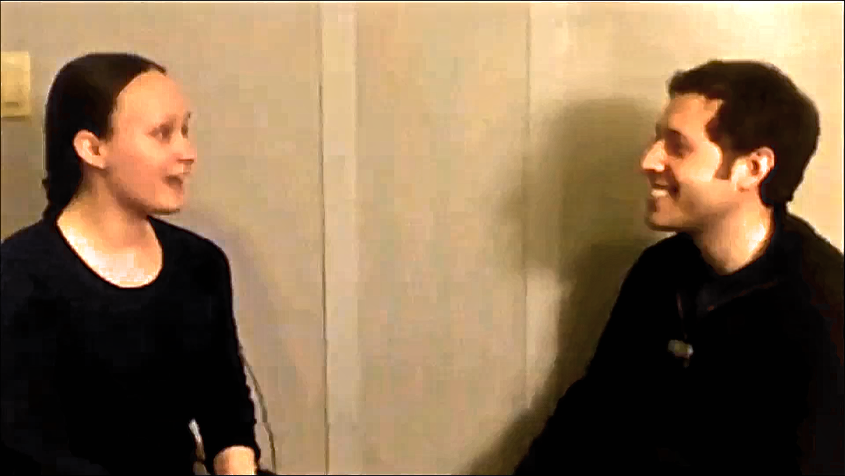
\includegraphics[width=0.6\textwidth]{figures/FIG-FL-stim.png}
\end{center}
\caption{Example frame from a conversation video used in Experiment 1.} 
\label{fig:speakers}
\end{figure}

\subsubsection{Materials}

\textit{Video recordings}. We recorded pairs of talkers while they conversed in a sound-attenuated booth (see sample frame in Figure \ref{fig:speakers}). Each talker was a native speaker of the language being recorded, and each talker pair was male-female. Using a Marantz PMD 660 solid state field recorder, we captured audio from two lapel microphones, one attached to each participant, while simultaneously recording video from the built-in camera of a MacBook. The talkers were volunteers, all members of the local post-graduate community, and were acquainted with their recording partner ahead of time. 

Each recording session began with a 20-minute warm-up period of spontaneous conversation during which the pair talked for five minutes on four topics (favorite foods, entertainment, hometown layout, and pets). Then we asked talkers to choose a new topic---one relevant to young children (e.g., riding a bike, eating breakfast)---and to improvise a dialogue on that topic. We asked them to speak as if they were on a children's television show in order to elicit child-directed speech toward each other. We recorded until the talkers achieved at least 30 seconds of uninterrupted discourse with enthusiastic, child-directed speech. Most talker pairs took less than five minutes to complete the task, usually by agreeing on a rough script at the start. We encouraged talkers to ask at least a few questions to each other during the improvisation. The resulting conversations were therefore not entirely spontaneous, but were as close as possible while still remaining child-oriented in topic, prosodic pattern, and lexicosyntactic construction.\footnote{All of the non-English talkers were fluent in English as a second language, and some fluently spoke a third or more language. We chose male-female pairs as a natural way of creating contrast between the two talker voices. See the videos here: NOTE: add link.}

After recording, we hand-aligned the audio and video files, and cropped each recording to the 30-second interval with the most turn activity. Because we recorded the conversations in stereo, the male and female voices came out of separate speakers during video playback. This gave each voice in the videos a localized source (from the left or right loudspeaker). We coded each turn transition in the videos for language group (English vs. non-English), inter-turn gap duration (in milliseconds), and speech act (question vs. non-question). The non-English stimuli were coded for speech act from a monolingual English-speaker's perspective, i.e., which turns ``sound like'' questions, and which don't. The coding for speech act in non-English videos was completed independently by two coders and then checked and discussed for agreement.

Because the conversational stimuli were recorded semi-spontaneously, the duration turn transitions and the number of speaker transitions in each video was variable. We measured the duration of each turn transition from the audio recording associated with each video. We excluded turn transitions longer than 550 msec and shorter than 0 msec (those with transitional overlap) from analysis.\footnote{Overlap occurs when an addressee begins a new turn before the current turn is finished. When overlap occurs, observers cannot switch their gaze in anticipation of the response because the response begins \textit{earlier} than expected; participants expect conversations to proceed with ``one speaker at a time'' \citep{sacks1974}. As such, they would still be fixated on the prior speaker when the overlap started, and then would have to switch their gaze \textit{reactively} to the responder.} This left approximately equal numbers of turn transitions available for analysis in the English (N$=$22) and non-English (N$=$21) videos. On average, the inter-turn gaps for English videos (mean$=$273 msec, median$=$291 msec) were slightly longer than for non-English videos (mean$=$226 msec, median$=$205 msec). The longer gaps in the English videos could give them a slight advantage: our definition of an ``anticipatory gaze shift'' includes shifts that are initiated during the gap between turns (Figure \ref{fig:criterion}), so participants had slightly more time to make anticipatory shifts in the English videos.

Questions made up approximately half of the turn transitions in the English (54\%; N$=$12) and non-English (48\%; N$=$10) videos. In the English videos, inter-turn gaps were slightly shorter for questions (mean$=$271 msec, median$=$254 msec) than non-questions (mean$=$276 msec, median$=$300 msec). The opposite was true for the non-English videos: question transitions (mean$=$264 msec, median$=$257 msec) had longer inter-turn gaps than non-question transitions (mean$=$191 msec, median$=$168 msec). Thus non-question (i.e., declarative) transitions in non-English videos were the briefest type of turn transition in the stimuli on average.

\subsubsection{Procedure} 
Participants sat in front of an SMI 120Hz corneal reflection eye-tracker mounted beneath a large flatscreen display. The display and eye-tracker were secured to a table with an ergonomic arm that allowed the experimenter to position the whole apparatus at a comfortable height, approximately 60 cm from the viewer. We placed stereo speakers on the table, to the left and right of the display. 

Before the experiment started, we warned adult participants that they would see videos in several languages and that, though they weren't expected to understand the content of non-English videos, we \textit{would} ask them to answer general, non-language-based questions about the conversations. Then after each video we asked participants one of the following randomly-assigned questions: ``which speaker talked more?'', ``which speaker asked the most questions?'' ``which speaker seemed more friendly?'', and ``did the speakers' level of enthusiasm shift during the conversation?'' We also asked if the participants could understand any of what was said after each video. The participants responded verbally while an experimenter noted their responses.

Children were less inclined to simply sit and watch videos of conversation in languages they didn't speak, so we used a different procedure to keep them engaged. The experimenter started each session by asking the child about what languages he or she could speak, and about what other languages he or she had heard of. Then the experimenter expressed her own enthusiasm for learning about new languages, and invited the child to watch a video about ``new and different languages'' together. If the child agreed to watch, the experimenter and the child sat together in front of the display, with the child centered in front of the tracker and the experimenter off to the side. If the child began to look bored during video playback, the experimenter would talk during the filler videos, either commenting on the previous conversation (``That was a neat language!'') or giving the language name for the next conversation (``This next one is called Hebrew. Let's see what it's like.''). The experimenter's comments reinforced the video-watching as a joint task.

All participants (child and adult) completed a five-point calibration routine before the first video started. We used a dancing Elmo for the children's calibration image. During the study, participants watched all six 30-second conversation videos with 15--30 second filler videos in-between them (e.g., running puppies, singing muppets, flying bugs). The first and last conversations were in American English and the intervening conversations were Hebrew, Japanese, German, and Korean. The presentation order of the non-English videos was shuffled into four lists, which participants were assigned to randomly. The entire experiment, including instructions, took 10--15 minutes.

\subsubsection{Data preparation and coding}
\label{sec:algorithm}

To determine whether participants predicted upcoming turn transitions, we needed to define a set of criteria for what counted as an anticipatory gaze shift. Prior work using similar experimental procedures has found that adults and children make anticipatory gaze shifts to upcoming talkers within a wide time frame; the earliest shifts occur before the end of the prior turn, and the latest occur after the onset of the response turn, with most shifts occurring in the inter-turn gap (Keitel et al., 2013; Hirvenkari, 2013; Tice and Henetz, \citeyear{TiceHenetz11}). Following prior work, we measured how often our participants shifted their gaze from the prior to the upcoming speaker \textit{before} the shift in gaze could have been initiated in reaction to the onset of the speaker's response. In doing so, we assumed that it takes children 333 msec to plan an eye movement, following Fernald and colleagues' (2008) similar `looking while listening' method.

We checked each participant's gaze at each turn transition for three characteristics: (1) that the participant fixated on the prior speaker for at least 100 msec at the end of the prior turn, (2) that sometime thereafter the participant switched to fixate on the upcoming speaker for at least 100 ms, and (3) that the switch in gaze was initiated within the first 333 msec of the response turn, or earlier. These criteria guarantee that we only counted gaze shifts when: (1) participants were tracking the previous speaker, (2) switched their gaze to track the upcoming speaker, and (3) did so before they could have simply reacted to the onset of speech in the response. Under this assumption, a gaze shift that is initiated within the first 333 msec of the response (or earlier) was planned \textit{before} the child could react to the onset of speech itself. For adult participants we used 200 msec (instead of 333 msec) as the assumed time to plan an eye movement.

\begin{figure}[t]
\begin{center}
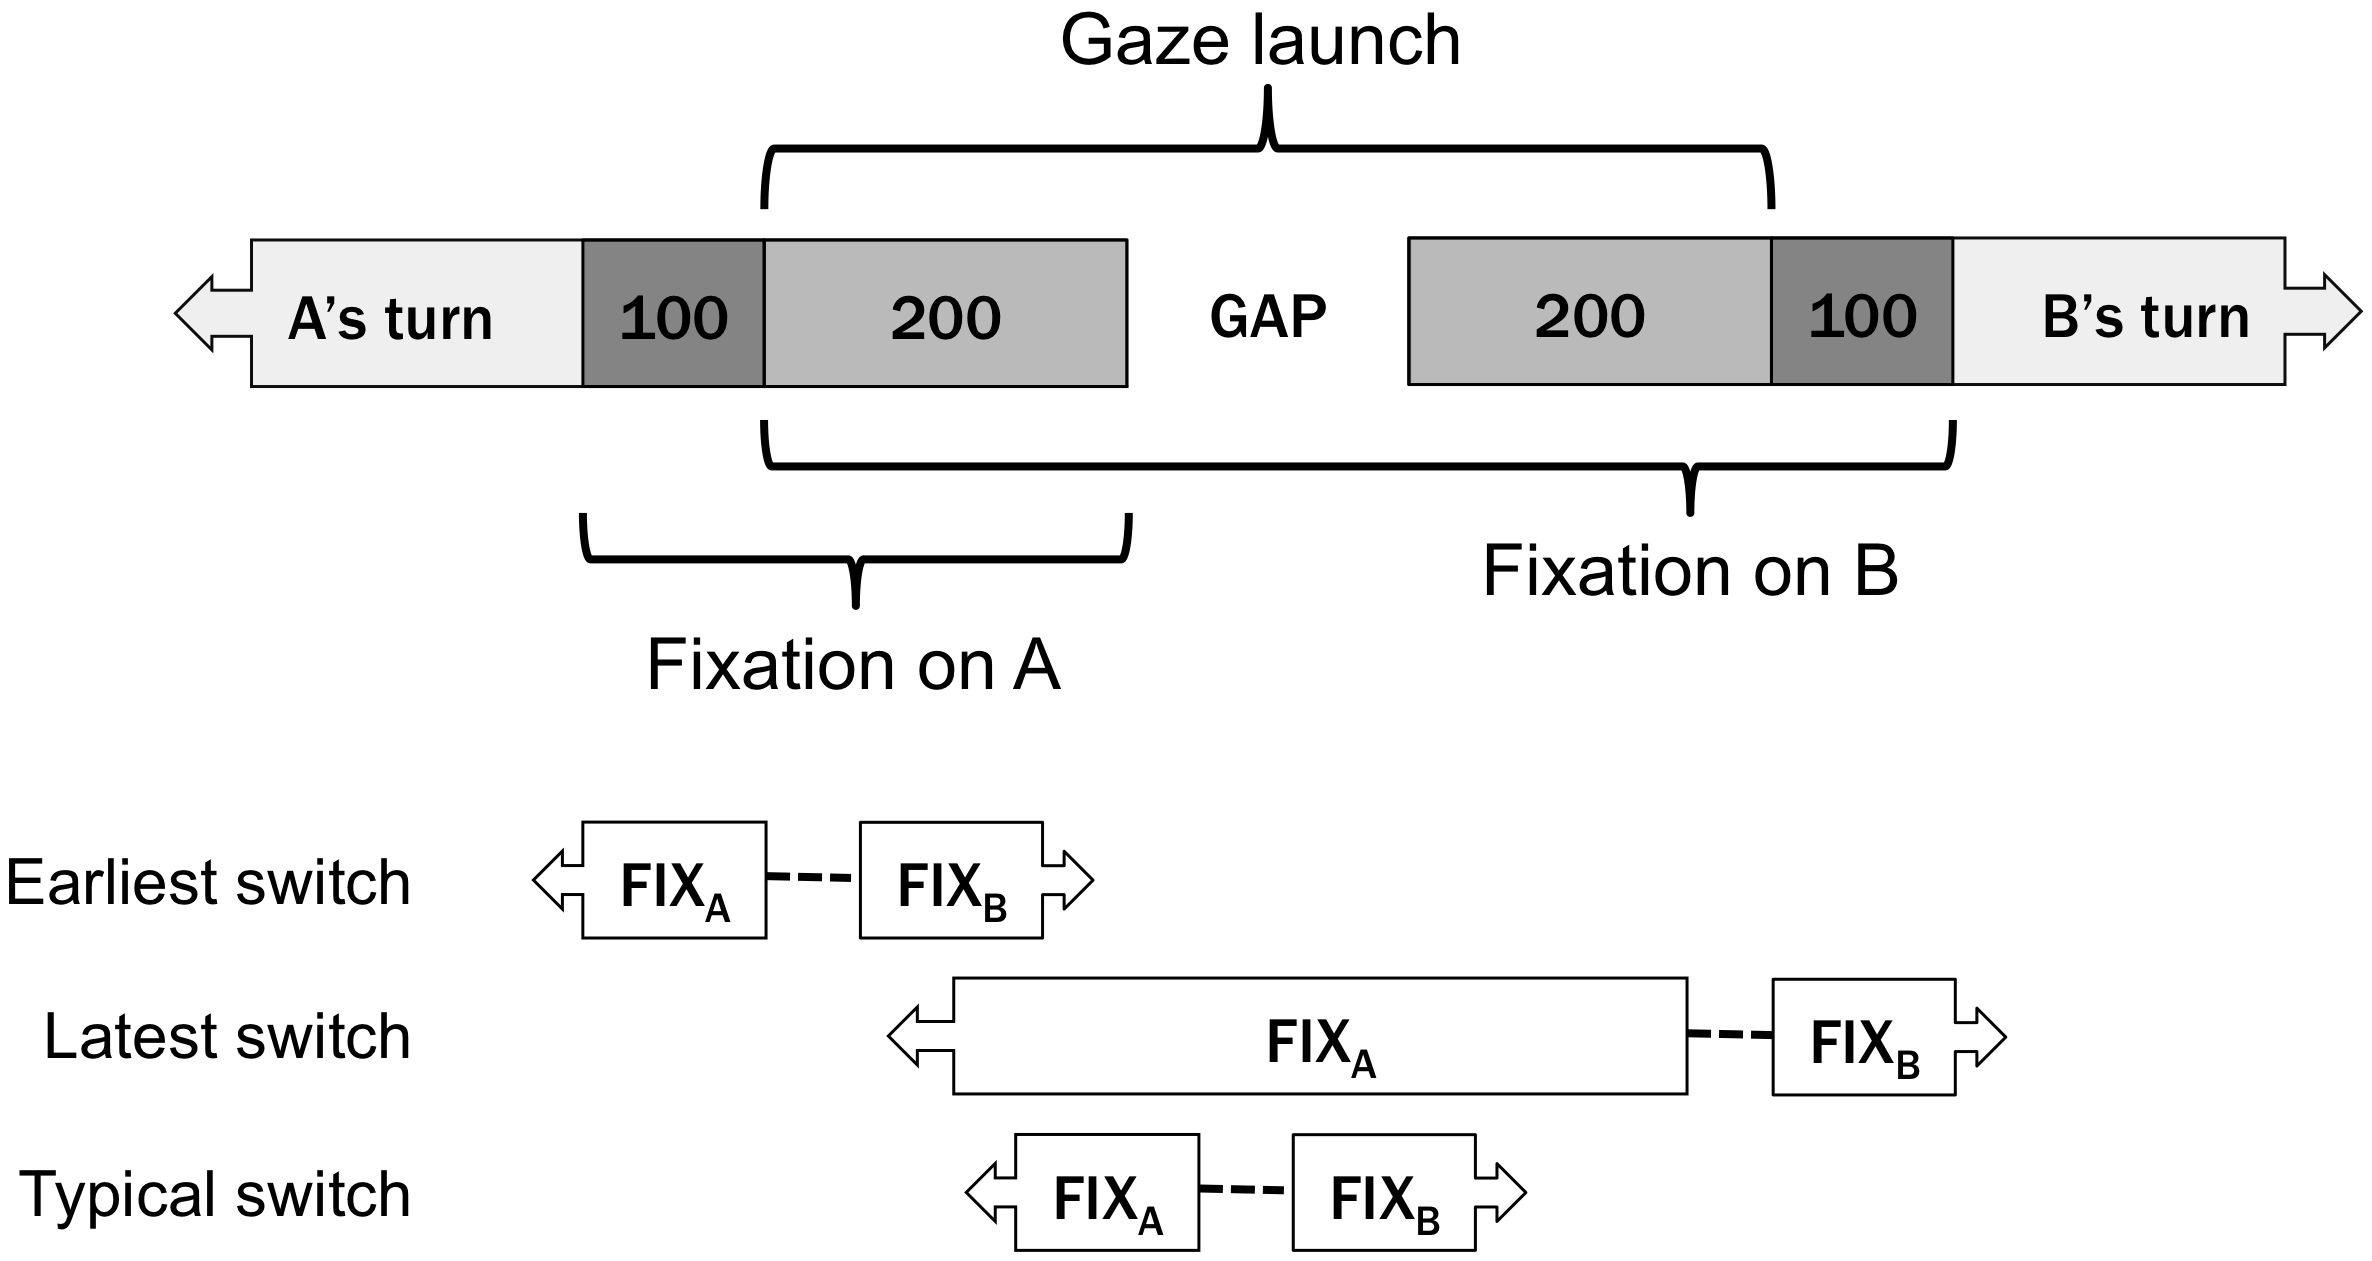
\includegraphics[width=0.7\textwidth]{figures/FIG-AnticipCriteria.png}
\end{center}
\caption{Schematic summary of criteria for anticipatory gaze shifts from speaker A to speaker B during a turn transition. The criteria were the same for adults and children, except children were assumed to have a 333 msec window for planning eye movements, while adults were only given 200 msec.} 
\label{fig:criterion}
\end{figure}

Using these criteria, we created a three-step algorithm for detecting anticipatory gaze switches. Consider, for example, when a child observes a turn transition between speaker A and speaker B (Figure \ref{fig:criterion}). First, the child would need to fixate on A for at least 100 msec at the end of A's turn. But what is the relevant window for fixation? Consistent with the distribution of responses in explicit turn-boundary prediction tasks (de Ruiter et al., 2006), we counted any early switches as ``truly turn-related'' as long as they occurred in the final 333 msec of A's turn (200 msec for adults). To allow for these early switches, the window for fixating on A must start 433 msec before the end of A's turn (300 msec for adults). Second, given that the child fixated on A, we checked to see if the child also fixated on B. Because we allowed for early switches, the first possible fixation on B could start 333 msec before the end of A's turn. Assuming that it took the child 333 msec to plan an eye movement, the latest point when the gaze could have \textit{anticipated} speech would be 333 msec after B's turn began---a switch after this point could simply be a reaction to the onset of B's speech. Thus, the relevant window for fixating on B started 333 msec before the gap and ended 433 msec after it (200 msec and 300 ms, respectively, for adults). Success on the first two criteria jointly implied that the child made an anticipatory switch in gaze. Our third step was to estimate when the switch occurred. Starting at a point when we knew participants were fixated on A (from step 1), we incremented forward in time to the first gaze measurement where the child looked away from A. We recorded the look-away timestamp as the time of gaze launch to the upcoming speaker.

\paragraph{Random baseline analysis} To ensure that participants' looking behavior was turn-related and not simply the result of random switching, we corrected for the probability of making an anticipatory switch at random. We estimated the baseline chance of making an anticipatory switch at each turn transition for each person. We ran all participants' eye-tracking data through switch identification with 100 randomly-shuffled versions of the original turn transition windows (Figure \ref{fig:shuffling}). For each of the 100 randomly-shuffled versions, we recorded and then averaged whether or not each participant made an anticipatory switch at each ``turn transition.'' We then subtracted the random baseline value from each participant's actual switch result (1 or 0) for each turn transition to arrive at the final, baseline-corrected values. Subtracting the random baseline this way can give us an estimate of how often participants switched above chance across ages, conditions, and transition types. If participants made the same number of anticipatory switches, regardless of turn transition location, there would be no evidence that their switching behavior was linked to the conversation stimulus. 

\begin{figure}[t]
\begin{center}
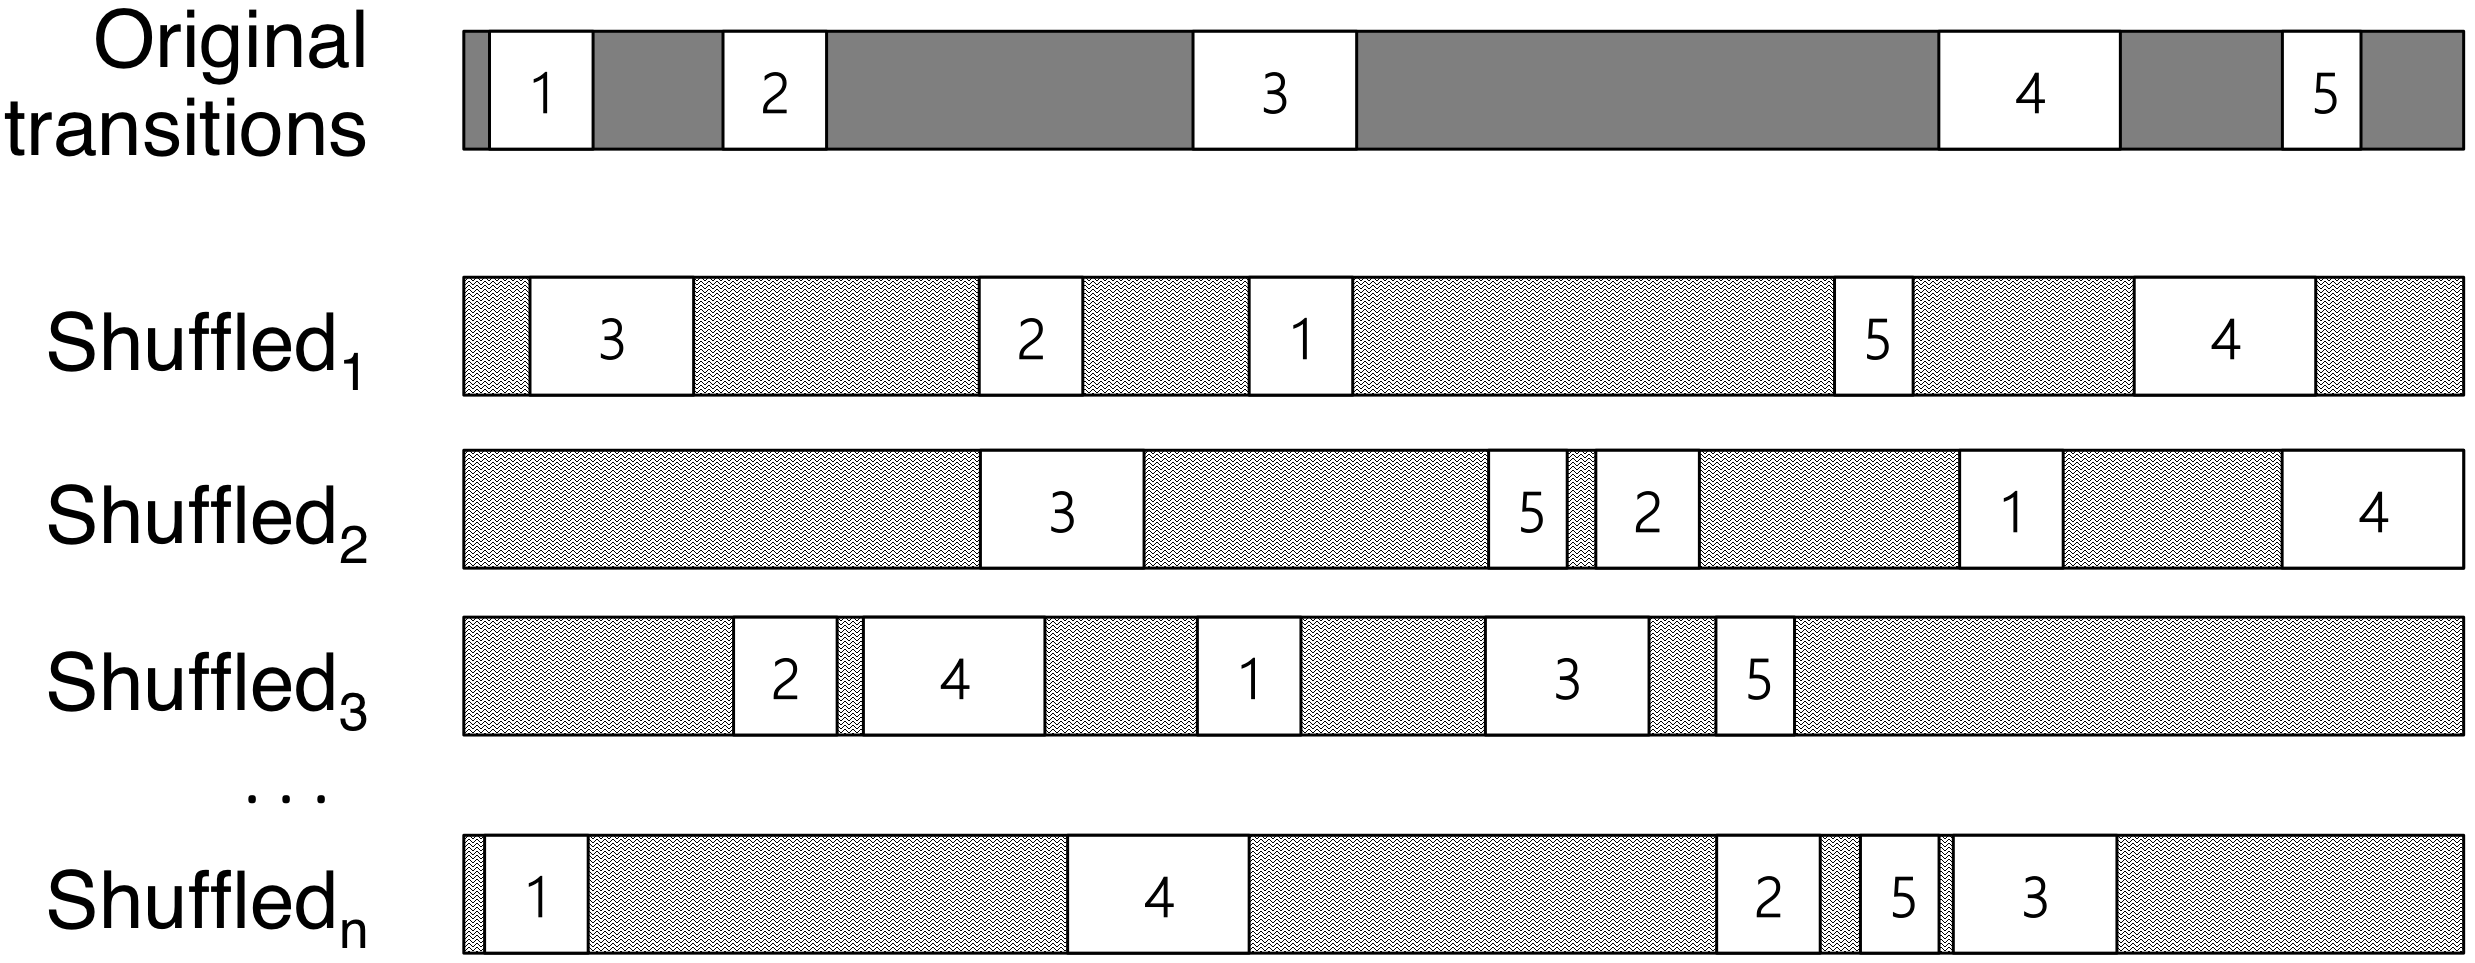
\includegraphics[width=0.6\textwidth]{figures/FIG-ShuffledWindows.png}
\end{center}
\caption{Example of shuffling for five turn transition windows. The windows were +/-433 msec around the inter-turn gap for children, and from +/-300 msec for adults.} 
\label{fig:shuffling}
\end{figure}

\subsection{Results and discussion}
\label{sec:results1}

\subsubsection{Descriptive analysis}

Participants looked at the screen most of the time during video playback (81\% and 91\% on average for children and adults, respectively). They primarily kept their eyes on the person who was currently speaking in both English and non-English videos: they gazed at the current speaker between 38\% and 63\% of the time, looking back at the addressee between 15\% and 20\% of the time (Table \ref{tab:e1_look}). Even three-year-olds looked more at the current speaker than anything else, whether the videos were in a language they could understand or not. Children looked at the current speaker less than adults did during the non-English videos. Despite this, their looks to the addressee did not increase substantially in the non-English videos, indicating that their looks away were probably related to boredom rather than confusion about ongoing turn structure. Overall, participants' pattern of gaze to current speakers indicated that they performed basic turn tracking during the videos, regardless of language.

\begin{table}[t]
\begin{center}
  \begin{tabular}{llcccc}
    \hline
    Age group & Condition & Speaker & Addressee & Other onscreen & Offscreen\\ 
    \hline
    3 & English & 0.61 & 0.16 & 0.14 & 0.08 \\ 
    4 & English & 0.60 & 0.15 & 0.11 & 0.13 \\ 
    5 & English & 0.57 & 0.15 & 0.16 & 0.12 \\ 
    Adult & English & 0.63 & 0.16 & 0.16 & 0.05 \\ 
    3 & Non-English & 0.38 & 0.17 & 0.20 & 0.25 \\ 
    4 & Non-English & 0.43 & 0.19 & 0.21 & 0.18 \\ 
    5 & Non-English & 0.40 & 0.16 & 0.26 & 0.18 \\ 
    Adult & Non-English & 0.58 & 0.20 & 0.16 & 0.07 \\ 
%   Overall & & 0.49 & 0.17 & 0.18 & 0.16 \\
    \hline
  \end{tabular}
\end{center}
  \caption{Average proportion of gaze to the current speaker and addressee during periods of talk.}
\label{tab:e1_look}
\end{table}

We identified anticipatory gaze switches for all 43 usable turn transitions, based on the criteria and algorithm outlined in Section \ref{sec:algorithm}. Because participants had greater access to lexical and syntactic information in English, we expected to see greater anticipation in the English videos than in the non-English videos. We also predicted that anticipation would be greater following questions compared to non-questions; questions have early cues to upcoming turn transition (e.g., \textit{wh-} words, subject-auxiliary inversion), and also make a next response immediately relevant. We also predicted that anticipatory looks would increase with development, along with children's increased linguistic competence.

To estimate the effects of linguistic condition and age on switching behavior, we corrected each participant's data by subtracting their random baseline estimations from their actual switching data for each turn transition. All comparisons below are made with the baseline-corrected values.

\begin{figure}[t]
\begin{center}
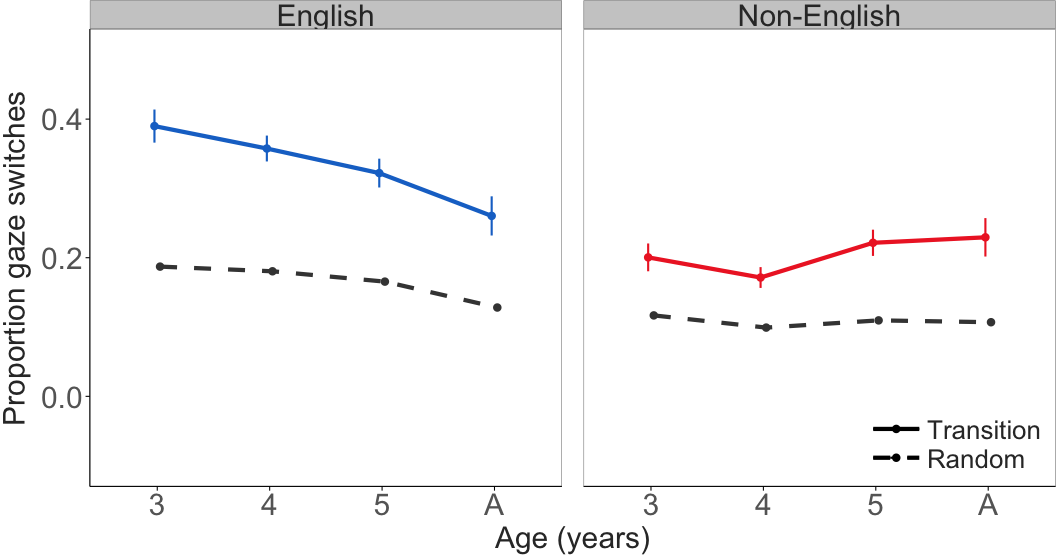
\includegraphics[width=0.8\textwidth]{figures/FIG-randvsreal-FL.png}
\end{center}
\caption{Proportion anticipatory gaze switches made for actual (solid) and randomly-shuffled (dashed) turn transitions in each condition, and across ages. Error bars represent the standard error of the mean.} 
\label{fig:randvsrealFL}
\end{figure}

Participants at all ages made anticipatory gaze switches more often than would be expected by chance, whether they could understand the language in the video or not (Figure \ref{fig:randvsrealFL}). Anticipatory switch behavior in the non-English videos could not have been based on lexicosyntactic information, so both adults and children must have relied on other sources of information to make their predictions (e.g., prosody and non-verbal signals).

Overall, a greater proportion of participants made anticipatory switches in the English videos (0.17) compared to the non-English videos (0.09). But the tendency to make more anticipatory switches for English than non-English videos disappeared with age. While anticipatory switches increased with age for non-English videos, they decreased with age for English videos, resulting in nearly equal looking behavior for the two language conditions for adults. Otherwise, age-based differences in predictive gaze shifts were minor (Figure \ref{fig:conditionsFL}).

\begin{figure}[t]
\begin{center}
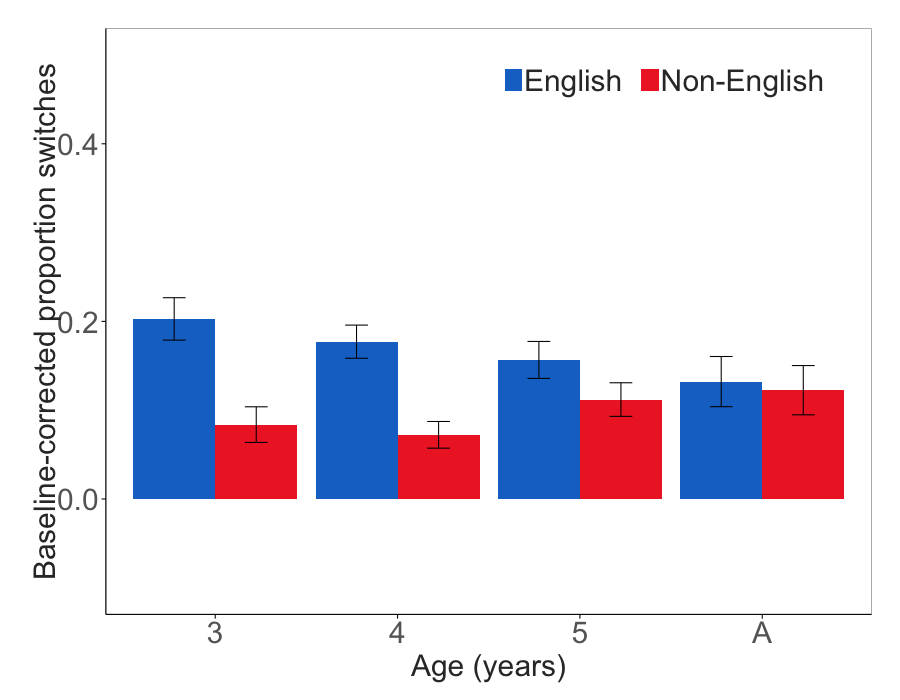
\includegraphics[width=0.5\textwidth]{figures/FIG-conditions-FL.png}
\end{center}
\caption{Baseline-corrected proportion anticipatory gaze switches made for turn transitions in each language condition, and across ages. Error bars represent the standard error of the mean.} 
\label{fig:conditionsFL}
\end{figure}

\begin{figure}[t]
\begin{center}
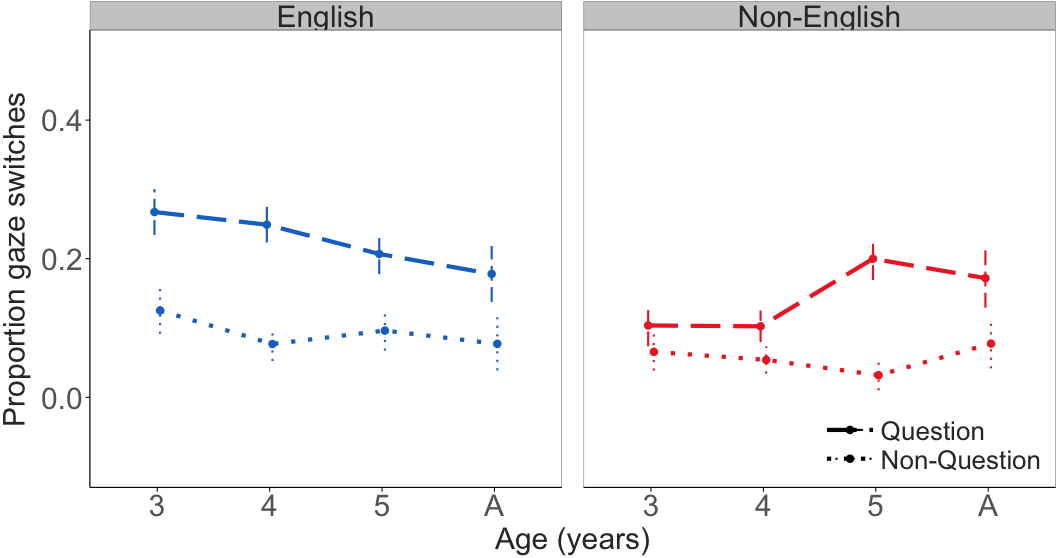
\includegraphics[width=0.8\textwidth]{figures/FIG-QvsNQ-FL.png}
\end{center}
\caption{Proportion anticipatory gaze switches made for question- (dashed) and non-question- (dotted) turn transitions in each condition, and across ages. Error bars represent the standard error of the mean.} 
\label{fig:questionsFL}
\end{figure}

Participants also showed an advantage for questions. Children made anticipatory switches twice as often when they heard a question, compared to a non-question (18.7\% and 7.3\%). But the advantage for questions was not universal---it depended on language condition and age. The advantage for questions didn't emerge until age five in the non-English videos (Figure \ref{fig:questionsFL}).

\subsubsection{Statistical analysis}

We quantified these findings using two linear mixed-effects models of baseline-corrected anticipatory switches \citep{lme4, R}. We built one model each for children and adults. The child model included condition (English vs. non-English)\footnote{Because each non-English language was represented by a single stimulus, we cannot compute reliable cross-language differences. Gaze behavior might be best for languages that have more structural overlap English. English speakers can make predictions about the strength of upcoming Swedish prosodic boundaries nearly as well as Swedish speakers do, but Chinese speakers are at a disadvantage in the same task \cite{carlson2005}. We would need multiple items from each of the language to check for similarity effects of specific linguistic features.}, transition type (question vs. non-question), age, and duration of the inter-turn gap as predictors, with full interactions between condition, transition type, and age.  We included the duration of the inter-turn gap as a predictor since longer gaps also provide more opportunities to make anticipatory switches (Figure \ref{fig:criterion}). We additionally included random effects of item (turn transition) and participant, with random slopes of condition, transition type, and their interaction for participants \citep{barr2013}. The adult model was exactly the same as the children's, excluding age-related effects.

Children's anticipatory gaze switches showed a main effect of language condition (\textit{$\beta$}=-0.448, \textit{SE}=0.126, \textit{t}=-3.56). As predicted, children made more anticipatory looks while they were watching videos that they could understand. In the English videos, children had access to lexicosyntactic information, which could have helped them make better predictions about upcoming turn structure. Although children performed better on the English videos, lexicosyntactic information was not exclusively responsible for their anticipatory switches; children still performed remarkably well when no lexical information was present at all, and even three-year-olds made anticipatory switches at an above-chance rate in the non-English videos.

Contrary to our expectation, there was no main effect of age (\textit{$\beta$}=-0.03, \textit{SE}=0.027, \textit{t}=-1.145). Children's anticipatory switches \textit{did} increase with age for the non-English videos, but it also decreased with age for the English videos, resulting in a significant interaction of age and language condition (\textit{$\beta$}=0.083, \textit{SE}=0.027, \textit{t}=3.063). We had expected that, as children got older, they would also show more anticipatory switches. But this is contradicted by decreased looks with age for English videos, which even extended to the adult data. One possible explanation is that older children and adults found the videos in English easy to comprehend, and so tracked the conversation less closely. Compared to three-year-olds, adults and older children spent more time looking away from the current speaker and addressee in the English conversations. In contrast, compared to three-year-olds, they spent more time looking at the current speaker and less time looking away in the non-English conversations (Table \ref{tab:e1_look}).

It is also possible that the timing of anticipatory gaze switches changes as children get older. That is, the moment at which observers chose to launch their gaze away from the current speaker might change with age. For example, children could have reacted more immediately to early cues in the turn (e.g., ``Which one...'') as they got older. If a change in timing were sufficiently large, we might not capture it in our analysis window, which was designed to capture switches close to the turn transition. To test for a change in switch timing, we would have to run new analyses on a larger set of turn transitions---ones with controlled early and late cues \citep[see, e.g.,][]{bogelsmagyariInPrep}. Within the current analysis windows there were some ``early switches'' (i.e., those launched before the end of the prior turn). But participants made approximately equal numbers of early switches, regardless of age and condition: 11--15\% (Figure \ref{fig:cumulativeFL}). The lack of increased early switching with age might suggest that changes in timing are either larger than the analysis window, or are not at play.

\begin{figure}[t]
\begin{center}
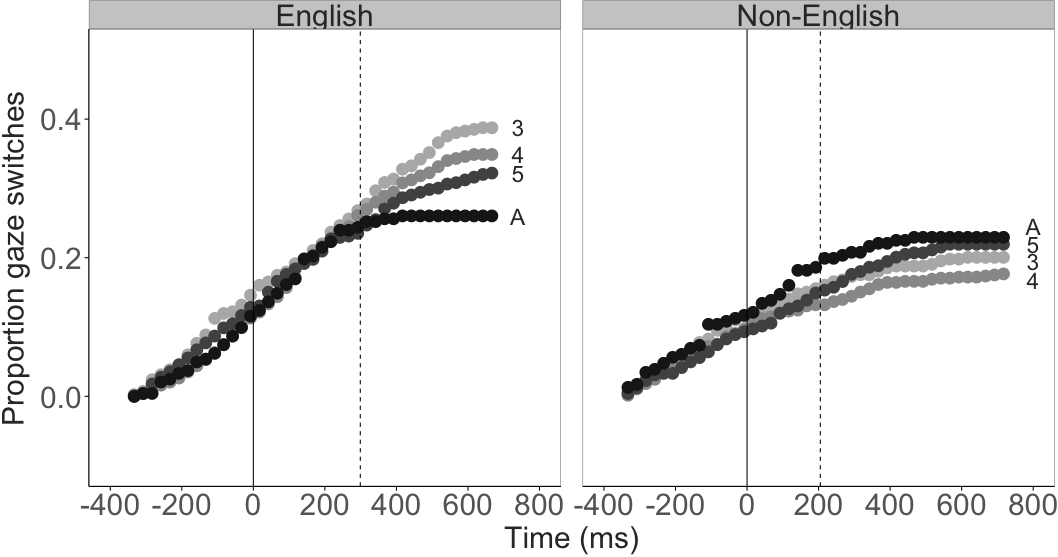
\includegraphics[width=0.8\textwidth]{figures/FIG-cumulative-FL.png}
\end{center}
\caption{Cumulative proportion of anticipatory gaze switches planned during the transition window, across conditions and ages. Age is indicated by hue (light to dark; darker = older). The solid line is the offset of the pre-gap turn, and the dashed line is the median onset of the post-gap turn in each condition. ``Early switches'' occur before 0.} 
\label{fig:cumulativeFL}
\end{figure}

Children made more anticipatory switches after hearing questions than non-questions, but the advantage for questions was driven by age and linguistic access. There was no main effect of transition type alone (\textit{$\beta$}=-0.209, \textit{SE}=0.151, \textit{t}=-1.384). Rather, the model confirmed a two-way interaction of linguistic condition and transition type (\textit{$\beta$}=0.445, \textit{SE}=0.19, \textit{t}=2.344). Presumably, question effects were larger in the English videos than the non-English videos because there were more cues to questionhood in English (i.e., non-verbal, prosodic, \textit{and} lexicosyntactic). Children younger than five did not distinguish questions from non-questions in the non-English videos (Figure \ref{fig:questionsFL}). The children's model confirmed a three-way interaction of age, linguistic condition, and transition type (\textit{$\beta$}=-0.091, \textit{SE}=0.042, \textit{t}=-2.183). Lexicosyntactic information might then be critical for young children to identify questions in conversation. Cues like subject-auxiliary inversion, and \textit{wh}-words occur early in the turn and are clear indicators that an answer will come next. Importantly, the turns marked as ``questions'' in the non-English data were not real questions, but turns that \textit{sounded like} questions to native English speakers. Question-like prosodic cues in the non-English videos could have been markedly different from question prosody in English, making it more difficult for three- and four-year-olds to identify ``questions'' in those conversations.

The increased switching after questions indicates that, so long as they have native lexical and prosodic cues, children as young as three spontaneously distinguish questions from other types of speech acts in third-party conversation. Children may treat questions differently from non-questions in conversation because they are predictably followed by an immediate response (i.e., the answer). Because the form of an answer is partially determined by its question (e.g., locative expressions for ``where'' questions), children could even be predicting what type of response they will hear, and look at the responder for confirmation. In contrast, non-questions do not usually require an immediate response, so it is not as easy to predict what will come next.

Inter-turn gap duration did not affect children's anticipatory switches (\textit{$\beta$}=0.202, \textit{SE}=0.151, \textit{t}=1.340), but it was the main factor driving adults' switches (\textit{$\beta$}=0.648, \textit{SE}=0.047, \textit{t}=13.855). The adult model also showed a marginal effect of transition type, with adults looking more after questions compared to non-questions (\textit{$\beta$}=-0.117, \textit{SE}=0.069, \textit{t}=-1.704). Language condition and its interaction with transition type were not significant. Language did not affect adults' anticipatory looking behavior, possibly because the animated, child-directed prosody and non-verbal cues made it possible for them to follow the interaction and track the current speaker easily.

\subsubsection{Summary}

Several results from Experiment 1 were unexpected. First, we found no significant main effect of age in the children's data, and we saw very little difference between adults and children (besides the age-related interactions). It appears that, especially in English, children were as good at tracking the current speaker and anticipating upcoming turns as adults were. To find out when children first begin making spontaneous anticipatory looks to responders, younger participants are required. Experiment 2 thus includes a sample of one- and two-year-olds. 

Second, children, but not adults, showed an advantage for lexicosyntactic information in their anticipatory switches. An advantage for lexicosyntactic information is consistent with prior work on adult turn taking \citep{de-ruiter2006}, so it's curious that the adults did not show a difference in anticipatory switching between videos they did and did not understand. As mentioned above, it is likely that they used non-verbal cues to track the interactions and consequently found the videos so easy to follow that they did not track the turn-taking closely. To identify which \textit{linguistic} cues adults and children rely on, it is necessary to control the presence of non-verbal cues in the stimulus---Experiment 2 implements this control.

Finally, we had predicted that children would show early advantages for prosodic cues over syntactic ones because children begin developing language-specific knowledge about prosody long before lexicosyntax. We weren't able to directly test this prediction in Experiment 1 because we used a limited range of ages (three- to five-year-olds) and because we only controlled for lexicosyntactic information. Children had prosodic cues in both English and non-English videos, although the prosodic signal was non-native in the latter case. So, although using non-English videos was a natural way to control for lexical information, it did not allow for assessment of the role of prosody. Relatedly, the advantage for questions was greater in the English videos than the non-English videos, suggesting that lexicosyntactic cues are important for children in identifying questions during conversation. Again, to test this idea, we would need to directly compare lexicosyntactic and prosodic cues in the participants' native language. In sum, the current study lays the analytic groundwork for a method that allows for greater experimental control, which we introduce in Experiment 2. 


%%%%%%%%%%%%%%%%%%%%%%%%%%%%%%%%%%%%%%%%%
%%%%%%%%%%%%%%%%%%%%%%%%%%%%%%%%%%%%%%%%%
%%%%%%%%%%%%%%%%%%%%%%%%%%%%%%%%%%%%%%%%%
%%%%%%%%%%%%%%%%%%%%%%%%%%%%%%%%%%%%%%%%%
%%%%%%%%%%%%%%%%%%%%%%%%%%%%%%%%%%%%%%%%%


\section{Experiment 2}
\label{sec:exp2}

We improved our design by using native-language stimuli, controlling for lexical \textit{and} prosodic information, eliminating non-verbal cues, and testing children from a wider age range. All of the videos in Experiment 2 were in the participants' native language (American English). To tease apart the role of lexical and prosodic information, we phonetically manipulated the speech signal for pitch, rhythm, and lexical access. By testing one- to six-year-olds we hoped to find the developmental onset of turn-predictive gaze. We also hoped to measure changes in the relative roles of prosody and lexicosyntax across development.

Non-verbal cues in Experiment 1 (e.g., gaze and gesture) could have helped participants make predictions about upcoming turn structure  \citep{rossano2009, stivers2010}. Since our focus is on linguistic cues, we eliminated all gaze and gestural signals in Experiment 2 by replacing the videos of human actors with videos of puppets. Puppets are less realistic and expressive than human actors but, since we wanted to eliminate gestural and gaze cues, the puppets created a natural context for having somewhat motionless talkers in the videos. Additionally, the prosody-controlled condition included small but global changes to syllable duration that would have required complex video manipulation or precise re-enactment with human talkers, neither of which was feasible. For these reasons, we decided to substitute puppet videos for human videos in the final stimuli. 

As in the first study, we recorded participants' eye movements as they watched six short videos of dyadic conversation, and then analyzed their anticipatory glances from the current speaker to the upcoming speaker at points of turn transition.

\subsection{Methods}
\label{sec:methods2}

\subsubsection{Participants}
We recruited 27 undergraduate adults and 129 children between ages 1;0--7;0 to participate in our study. We recruited our child participants from the Children's Discovery Museum in San Jose, California, targeting approximately 20 children for each of the six 1-year age groups (range$=$20--23). All participants were native English speakers, though some parents (N$=$27) reported that their child heard a second (and sometimes third) language at home. None of the adult participants reported fluency in a second language. We ran Experiment 2 at a local children's museum because it gave us access to children with a more diverse range of ages.

\begin{figure}[t]
\begin{center}
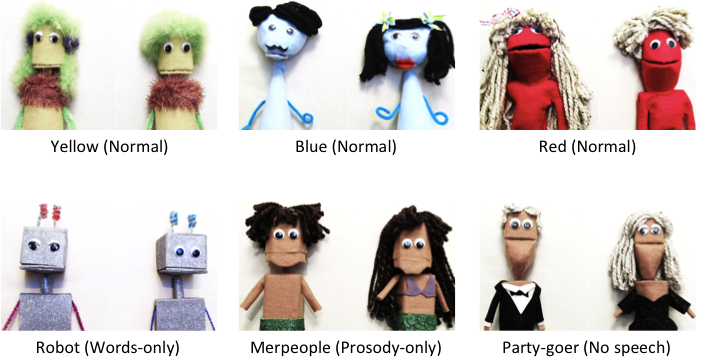
\includegraphics[width=0.9\textwidth]{figures/FIG-EN-stim.png}
\end{center}
\caption{The six puppet pairs (and associated audio conditions). Each pair was linked to three distinct conversations from the same condition across the three experiment versions.}
\label{fig:puppets}
\end{figure}

\subsubsection{Materials}
We created six short videos of improvised, child-friendly conversation (Figure \ref{fig:puppets}). To eliminate non-verbal cues to turn transition and to control the types of linguistic information available in the stimuli we (1) recorded improvised conversations, (2) phonetically manipulated those recordings to limit the availability of prosodic and lexical information, and (3) recorded a new set of videos that featured puppets as talkers, using the manipulated audio as the puppets' speech. 

\textit{Audio recordings}. The recording session was set up in the same way as the first study, but with a shorter warm up period (5--10 minutes) and a pre-determined topic for the child-friendly improvisation (`riding bikes', `pets', `breakfast', `birthday cake', `rainy days', or `the library'). All of the talkers were native English speakers, and were recorded in male-female pairs. As before, we asked talkers to speak ``as if they were on a children's television show'' and to ask at least a few questions during the improvisation. We cut each audio recording down to the 20-second interval with the most turn activity. The 20-second clips were then phonetically manipulated and used in the final video stimuli.

\textit{Audio Manipulation}. We created four versions of each audio clip: \textit{normal}, \textit{words only}, \textit{prosody only}, and \textit{no speech}. That is, one version with a full linguistic signal (\textit{normal}), and three with incomplete linguistic information (hereafter ``limited cue'' conditions). The \textit{normal} clips were the unmanipulated, original audio clips. 

The \textit{words only} clips were manipulated to have robot-like speech: we flattened the intonation contours to each talker's average pitch (F0) and we reset the duration of every nucleus and coda to each talker's average nucleus and coda duration.\footnote{We excluded hyper-lengthened words like [w\textipa{aU:}] `woooow!'. These were rare in the clips.} We made duration and pitch manipulations using PSOLA resynthesis in Praat \citep{Praat}. Thus, the \textit{words only} versions of the audio clips had no pitch or durational cues to upcoming turn boundaries, but did have intact lexicosyntactic cues. 

We created the \textit{prosody only} clips by low-pass filtering the original recording at 500 Hz with a 50 Hz Hanning window (following de Ruiter et al., 2006). This manipulation creates a ``muffled speech'' sound because low-pass filtering removes most of the phonetic information used to distinguish between phonemes. The \textit{prosody only} versions of the audio clips lacked lexical information, but retained their intonational and rhythmic cues to upcoming turn boundaries. 

The \textit{no speech} condition served as a non-linguistic baseline. For this condition, we replaced the original clip with multi-talker babble: eight different child-oriented conversations (\textit{not} including the original one), overlaid and cropped to the duration of the video. Thus, the \textit{no speech} audio clips lacked any linguistic information to upcoming turn boundaries---the only cue to turn-taking was the opening and closing of the puppets' mouths. 

Finally, because low-pass filtering removes significant acoustic energy, the \textit{prosody only} clips were much quieter than the other three conditions. Our last step was to downscale the intensity of videos from the three other conditions to match the volume of the \textit{prosody only} clips. We referred to the conditions as ``normal'', ``robot'', ``mermaid'', and ``birthday party'' speech when interacting with participants.

\textit{Video recordings}. We created puppet video recordings to match the manipulated 20-second audio clips. The puppets were minimally expressive; the experimenter could only control the opening and closing of their mouths; their head, eyes, arms, and body stayed still. Puppets were positioned looking forward to eliminate shared gaze as a cue to turn structure \citep{thorgrimssonUndRev}. We took care to match the puppets' mouth movements to the syllable onsets as closely as possible and avoided any mouth movement before the onset of a turn. We then hand-aligned the manipulated audio clips to the puppet video recordings.

We used three pairs of puppets used for the \textit{normal} condition---`red', `blue' and `yellow'---and one pair of puppets for each limited cue condition: ``robots'', ``merpeople'', and ``party-goers'' (Figure 8). We randomly assigned half of the conversation topics (`birthday cake', `pets', and `breakfast') to the \textit{normal} condition, and half to the limited cue conditions (`riding bikes', `rainy days', and `the library'). We then created three versions of the experiment, so that each of the six puppet pairs was associated with three different conversation topics across the different versions of the experiment. We ensured that the position of the talkers (left and right) was counterbalanced in each version by flipping the video and audio channels as needed.\footnote{See the videos here: FIX add link.}

The duration of turn transitions and the number of speaker changes across videos was variable because the conversations were recorded semi-spontaneously. We measured turn transitions from the audio recording of the \textit{normal}, \textit{words only}, and \textit{prosody only} conditions. There was no audio from the original conversation in the \textit{no speech} condition videos, so we measured turn transitions from the video recording, using ELAN video editing software \citep{ELAN}. 

There were 79 turn transitions for analysis, after excluding transitions longer than 550 msec and shorter than 0 msec. The remaining turn transitions were distributed evenly across transition types (questions N$=$47 and non-questions N$=$32) and conditions, keeping in mind that there were three \textit{normal} videos and only one limited cue video for each experiment version: \textit{normal} (N$=$36), \textit{words only} (N$=$13), \textit{prosody only} (N$=$12), and {no speech} (N$=$18). Question transitions (mean$=$358, median$=$405) were longer than non-question transitions (mean$=$296, median$=$288) on average, but gap duration was overall comparable across conditions: \textit{normal} (mean$=$333, median$=$337), \textit{words only} (mean$=$345, median$=$383), \textit{prosody only} (mean$=$320, median$=$336), and \textit{no words} (mean$=$324, median$=$328). The longer gaps for question transitions could give them an advantage because our anticipatory measure includes shifts initiated during the gap between turns (Figure \ref{fig:algorithm}).

\subsection{Procedure}
We used the same experimental apparatus and procedure as in the first study. Each participant watched six puppet videos in random order, with five 15--30 second filler videos placed in-between (e.g., running puppies, moving balls, flying bugs). Three of the puppet videos had \textit{normal} audio while the other three had \textit{words only}, \textit{prosody only}, and \textit{no speech} audio. This study required no special instructions so the experimenter immediately began each session with calibration (same as before) and then stimulus presentation. The entire experiment took less than five minutes.

\textit{Data preparation, coding, and random baseline analysis}. We coded each turn transition for its linguistic condition (\textit{normal}, \textit{words only}, \textit{prosody only}, and \textit{no speech}) and transition type (question/non-question)\footnote{We coded \textit{wh-}questions as ``non-questions'' for the \textit{prosody only} videos. Prototypical \textit{wh-}questions are not marked with a final rising nuclear prosodic contour, but polar questions are \citep{hedberg2010}.}, identified anticipatory gaze switches to the upcoming speaker, and estimated a random baseline of anticipatory switches using the methods from Experiment 1.

\subsection{Results and discussion}
\label{sec:results2}

\subsubsection{Descriptive analysis}
Participants' pattern of gaze indicated that they performed basic turn tracking across all ages and in all conditions. Participants looked at the screen most of the time during video playback (82\% and 86\% average for children and adults, respectively). Children and adults primarily kept their eyes on the person who was currently speaking: they gazed at the current speaker between 44\% and 69\% of the time, looking back at the addressee between 11\% and 14\% of the time (Table 2). They tracked the current speaker in every condition---even one-year-olds looked more at the current speaker than at anything else in the three limited cue conditions (40\% for \textit{words only}, 43\% for \textit{prosody only}, and 39\% for \textit{no speech}). There was a steady overall increase in looks to the current speaker with age and added linguistic information (Tables \ref{tab:look_e2} and \ref{tab:look_e2b}). Looks to the addressee also decreased with age, but the change was minimal. 

\begin{table}[t]
\begin{center}
  \begin{tabular}{llcccc}
    \hline
    Age group & Speaker & Addressee & Other onscreen & Offscreen\\ 
    \hline
    1 & 0.44 & 0.14 & 0.23 & 0.19 \\ 
    2 & 0.50 & 0.13 & 0.24 & 0.14 \\ 
    3 & 0.47 & 0.12 & 0.25 & 0.16 \\ 
    4 & 0.48 & 0.11 & 0.29 & 0.12 \\ 
    5 & 0.54 & 0.11 & 0.20 & 0.14 \\ 
    6 & 0.60 & 0.12 & 0.18 & 0.10 \\
    Adult & 0.69 & 0.12 & 0.09 & 0.10 \\
%   Overall & 0.53 & 0.12 & 0.21 & 0.13 \\
    \hline
  \end{tabular}
\end{center}
  \caption{Average proportion of gaze to the current speaker and addressee during periods of talk across ages.}
\label{tab:look_e2}
\end{table}

\begin{table}[t]
\begin{center}
  \begin{tabular}{llcccc}
    \hline
    Condition & Speaker & Addressee & Other onscreen & Offscreen\\ 
    \hline
    Normal & 0.58 & 0.12 & 0.17 & 0.13 \\ 
    Words only & 0.54 & 0.11 & 0.24 & 0.10 \\ 
    Prosody only & 0.48 & 0.12 & 0.26 & 0.15 \\ 
    No speech & 0.44 & 0.13 & 0.26 & 0.18 \\
    \hline
  \end{tabular}
\end{center}
  \caption{Average proportion of gaze to the current speaker and addressee during periods of talk across conditions.}
\label{tab:look_e2b}
\end{table}

% Average prop gaze to the current speaker across conditions for one-year-olds
%                           speaker addressee other-screen offscreen
%Normal   		  0.4737582 0.1366432    0.2003952 0.1892035
%Words only    0.3977261 0.1283417    0.3112005 0.1627317
%Prosody only 0.4290202 0.1611453    0.2558657 0.1539688
%No speech    0.3786925 0.1228615    0.2356423 0.2628037

We identified anticipatory gaze switches for all 79 usable turn transitions using the same criteria and algorithm as in Experiment 1. We expected to see the most anticipatory switches in the \textit{normal} condition and the least anticipatory switches in the \textit{no speech} condition because they contained the most and least linguistic information, respectively. We expected to replicate our finding that questions result in more anticipatory switches than non-questions, with the added hypothesis that the question effect is driven by lexicosyntactic cues. We also anticipated an overall increase in anticipatory switches with age. Finally, since the development of prosodic skills partially precedes the development of lexicosyntax, we expected to see more switches in the \textit{prosody only} condition compared to the \textit{words only} condition in the youngest age groups.

As in Experiment 1, we corrected each participant's gaze data by subtracting their random baseline from their actual switching for each turn transition. All comparisons below were made with the baseline-corrected values.

Participants at all ages made anticipatory gaze switches more often than would be expected by chance in almost all conditions, but sometimes by a small margin (Figure \ref{fig:randvsrealEN}). For example, anticipatory switches in the \textit{no speech} videos were often only modestly above chance (with the exception of 5- and 6-year-olds). Further, 1- and 2-year-olds did not appear to reliably outperform chance conditions for the \textit{words only} videos.

\begin{figure}[t]
\begin{center}
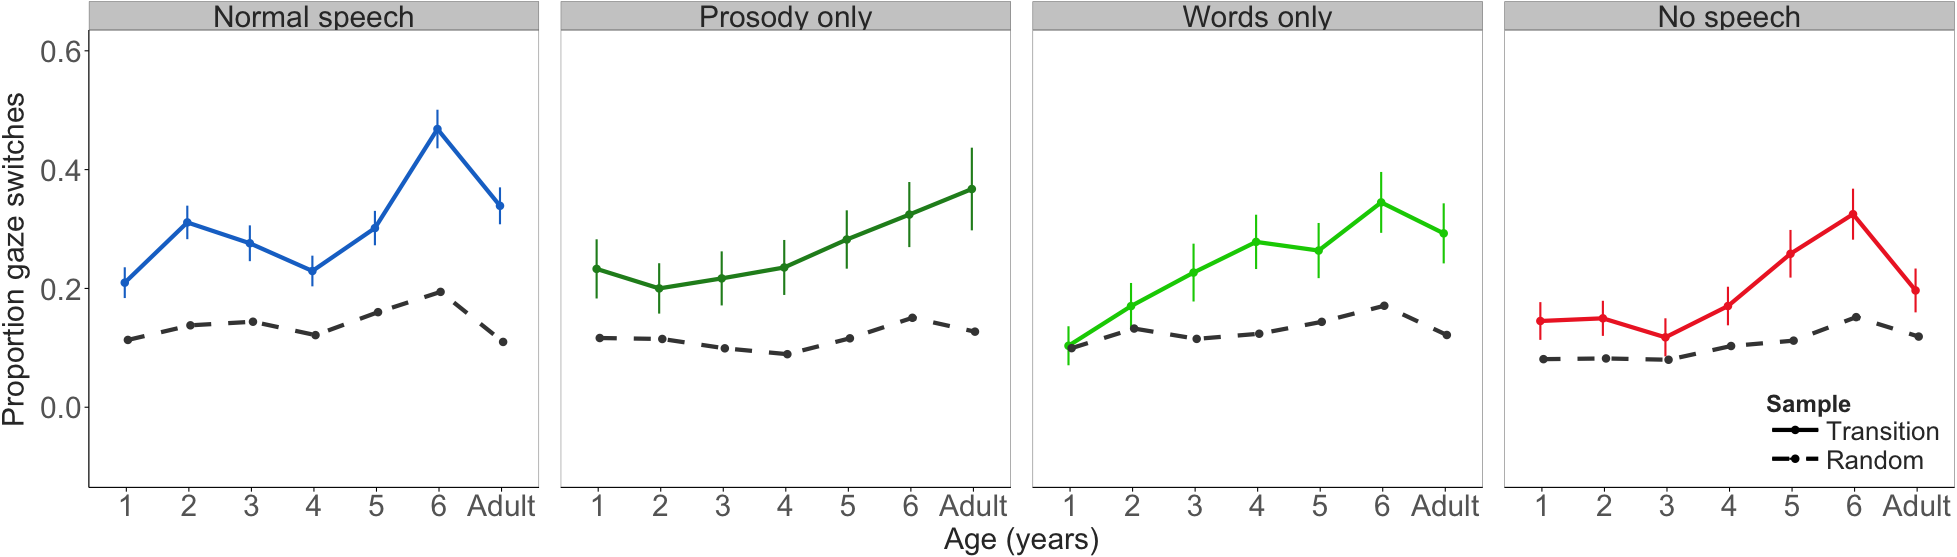
\includegraphics[width=0.99\textwidth]{figures/FIG-randvsreal-EN.png}
\end{center}
\caption{Baseline-corrected proportion anticipatory gaze switches made for actual (solid) and randomly-shuffled (dashed) turn transitions in each condition, and across ages. Error bars represent the standard error of the mean.} 
\label{fig:randvsrealEN}
\end{figure}

We observed that, overall, children and adults made the fewest anticipatory switches in the \textit{no speech} videos (9\%) and the most in the \textit{normal} videos (16\%), with the \textit{prosody only} and \textit{words only} videos falling in-between (14\% and 11\%, respectively; Figure \ref{fig:conditionsEN}). However, these condition-based differences were primarily driven by transition type effects (question vs. non-question).

\begin{figure}[t]
\begin{center}
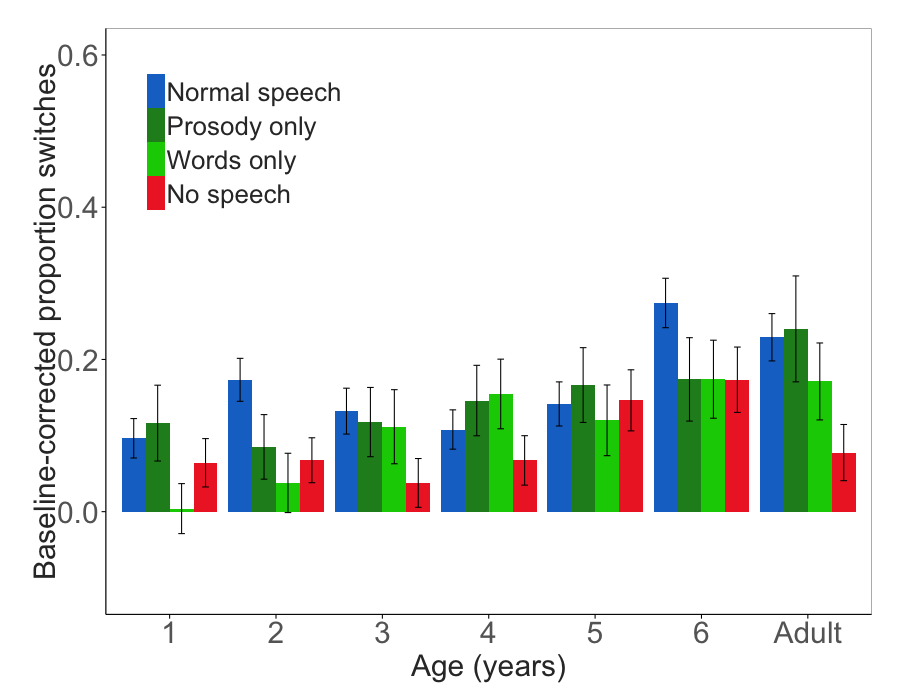
\includegraphics[width=0.65\textwidth]{figures/FIG-conditions-EN.png}
\end{center}
\caption{Proportion anticipatory gaze switches made for turn transitions in each speech condition, and across ages. Error bars represent the standard error of the mean.} 
\label{fig:conditionsEN}
\end{figure}

Participants made more anticipatory gaze switches following questions than non-questions, but only in the two lexical conditions (\textit{normal} and \textit{words only} speech). The advantage for questions was strongest in the \textit{normal} speech condition, where it emerged early in development. The question effect became larger with age in both lexical conditions. While children made small, sometimes non-linear, gains in their anticipatory switches for non-questions as they grew older, they made large gains in their anticipatory switches with age (especially between ages one and two; Figure \ref{fig:questionsEN}). The increased question effect from age one to two indicates that, around this age, children begin to leverage lexicosyntactic cues in the speech signal to identify questions in ongoing conversation. In the lexical conditions, children had access to early cues to questionhood, such as \textit{wh}-words and subject-auxiliary inversion, to predict an upcoming speaker change. In the \textit{normal} condition, where the question effect was strongest, lexical and syntactic cues were reinforced by question prosody for polar questions.

\begin{figure}[t]
\begin{center}
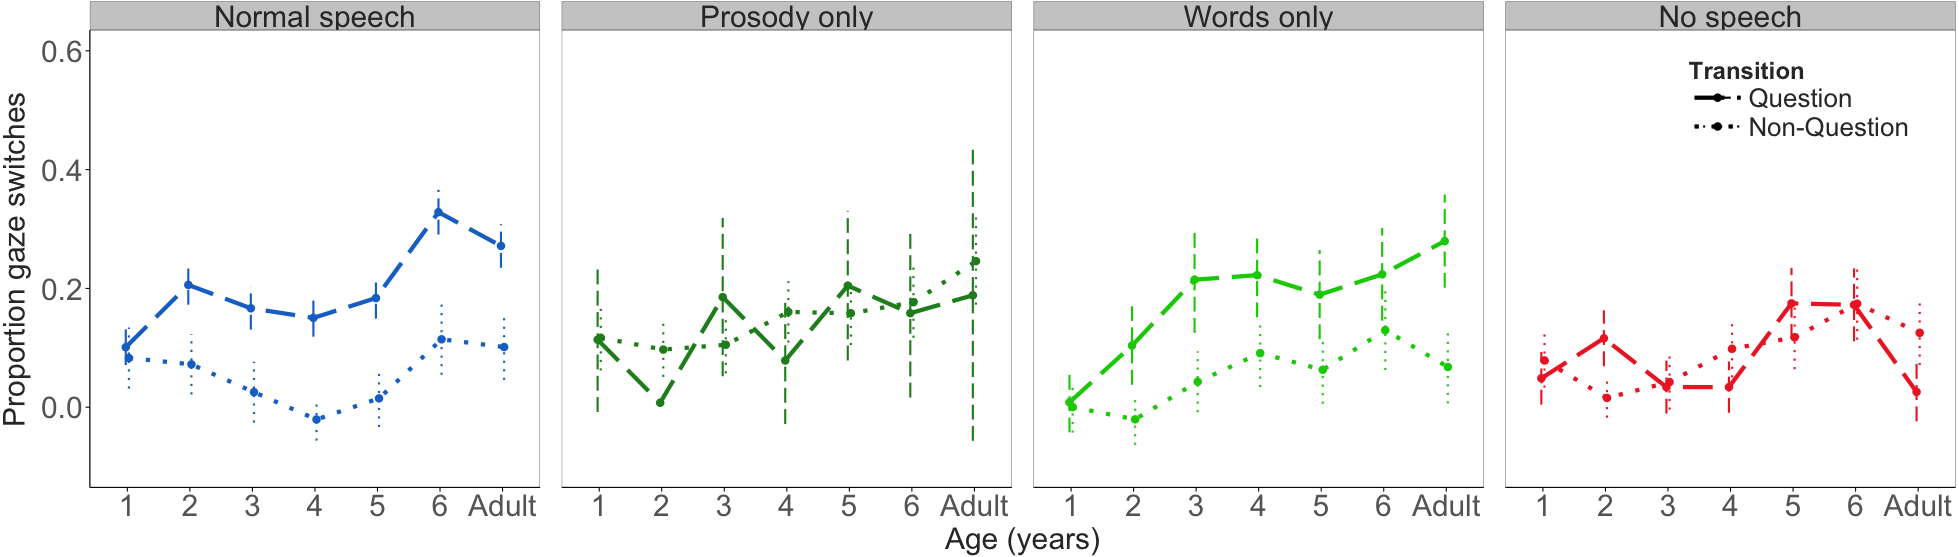
\includegraphics[width=0.99\textwidth]{figures/FIG-QvsNQ-EN.png}
\end{center}
\caption{Baseline-corrected proportion anticipatory gaze switches made for question- (dashed) and non-question- (dotted) turn transitions in each condition, and across ages. Error bars represent the standard error of the mean.} 
\label{fig:questionsEN}
\end{figure}

Notably, while children performed well with \textit{prosody only} speech from the start, they seemed to only reliably exceed chance in the \textit{words only} condition at ages 3;0 and older. We confirmed this pattern in two \textit{post-hoc} \textit{t}-tests comparing children's anticipatory switching rate against their estimated random switching rate before age 3;0. We found that children under 3;0 significantly exceeded chance for the \textit{prosody only} condition (\textit{t}(187.677)=-3.004, \textit{p}=.003), but not for the \textit{words only} condition (\textit{t}(229.828)=-0.8307, \textit{p}=.407), giving some support to the idea that there is an early advantage for prosody over lexicosyntax in children's turn prediction. All in all, children showed increases in anticipatory switching with age across all conditions. Adults reacted to the \textit{no speech} condition differently than the children did, tracking the interaction less closely than in the three linguistic conditions. They may have minimized switching in the \textit{no speech} condition because they realized that there was no conversation to follow.

\subsubsection{Statistical analysis}

We tested these findings in two linear mixed-effects models of the baseline-corrected anticipatory switches---one model each for children and adults. The child model included condition (\textit{normal}, \textit{words only}, \textit{prosody only}, and \textit{no speech}), transition type (question vs. non-question), age, and gap duration as fixed effects, with full interactions between condition, transition type, and age. The model also included random effects of item (turn transition) and participant, with random slopes of condition and transition type for participants. The adult model matched the child model, excluding age-related effects.

There was a significant effect of gap duration. Children had time to make more anticipatory switches in analysis windows with longer gaps (\textit{$\beta$}=0.294, \textit{SE}=0.091, \textit{t}=3.231). An effect of gap duration is expected since prior work using spontaneous anticipatory switching has found that most switches occur in the inter-turn gap (Keitel et al., 2013; Hirvenkari, 2013; Tice and Henetz, 2011).

Condition-related differences were driven by age and transition type (Figure \ref{fig:questionsEN}). Consequently, the model of children's anticipatory switches revealed no significant main effects of condition, despite the large changes in the linguistic information available across conditions. One interpretation of this finding is that children do not need linguistic information to predict upcoming turns. For example, children still made some anticipatory switches in the \textit{no speech} condition, even though the only cue to turn taking was the alternating mouth movements of the conversing puppets. With sufficiently long inter-turn gaps, participants could simply switch their gaze to the responder when the prior talker finishes talking---a strategy that doesn't rely on linguistic information. But this interpretation is not compatible with our finding that children make more anticipatory looks after hearing questions, that they do so more often when lexical information is available, and that they do even more so as they age.

The model of children's data confirmed two three-way effects of age, condition, and transition type. Children made significantly more anticipatory switches with age in the \textit{normal} (\textit{$\beta$}=0.04, \textit{SE}=0.008, \textit{t}=5.168) and \textit{words only} conditions (\textit{$\beta$}=0.031, \textit{SE}=0.01, \textit{t}=3.170): they made a switch twice as often after hearing a question (16\%) than a non-question (8\%) in the \textit{words only} condition, and nearly four times as often in the \textit{normal} condition (19\% vs. 5\%). Since the question effect was limited to the lexical conditions, there was no main effect of transition type. There were also no further interactions of age and condition, or of transition type and condition. There was, however, a significant two-way interaction of transition type and age (\textit{$\beta$}=-0.031, \textit{SE}=0.01, \textit{t}=-3.18), in addition to the three-way interactions for the \textit{normal} and \textit{words only} conditions already mentioned.

Last but not least, the model confirmed a significant main effect of age in the children's data (\textit{$\beta$}=0.028, \textit{SE}=0.009, \textit{t}=3.018). Children made more anticipatory switches as they got older. Many of the increased anticipatory looks with age came from questions in the lexical conditions. Children also increased their anticipatory looking with age for non-questions and non-lexical conditions, but the gains were smaller and sometimes followed a non-linear trajectory (Figure \ref{fig:questionsEN}). As in Study 1, early switches (planned before the end of the prior turn) did not show large increases with age, with adults making the fewest early switches in the three linguistic conditions (Figure \ref{fig:cumulativeEN}).

\begin{figure}[ht]
\begin{center}
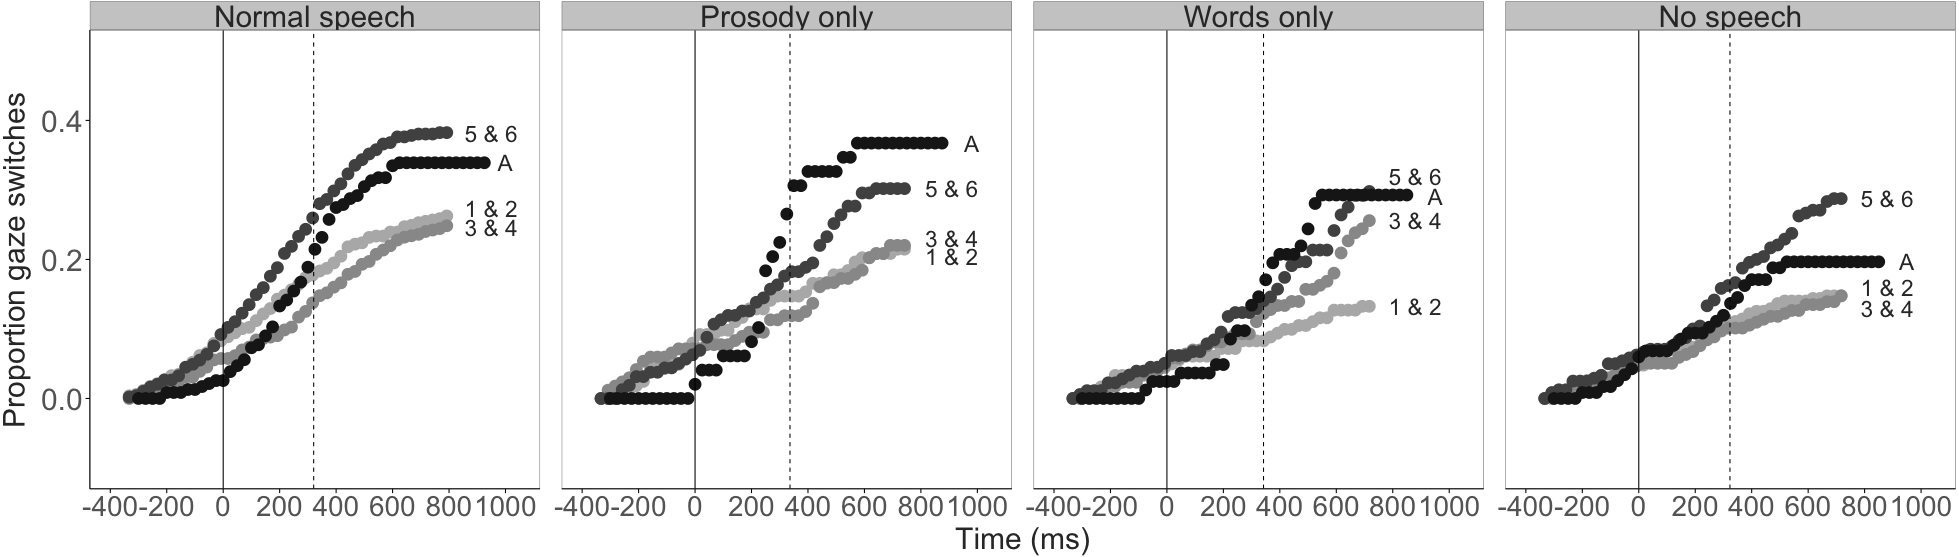
\includegraphics[width=0.99\textwidth]{figures/FIG-cumulative-EN.png}
\end{center}
\caption{Cumulative proportion of anticipatory gaze switches planned during the transition window, across conditions and ages. Age is indicated by hue (light to dark; darker = older). The solid line is the offset of the pre-gap turn, and the dashed line is the median onset of the post-gap turn in each condition. ``Early switches'' occur before 0.} 
\label{fig:cumulativeEN}
\end{figure}

The advantage for questions over non-questions in these results reinforces our findings from Study 1. They suggest that even two-year-olds can reliably distinguish questions from other transition types in third-party conversation, especially when full linguistic information is available. Inspecting the data more closely, we found that 43\% of one-year-olds made more anticipatory switches after questions than non-questions in the \textit{normal} condition, and 24\% of them did so in the \textit{words only} condition. Meanwhile, 61\% of two-year-olds show the effect in the \textit{normal} condition, and 52\% of them do in the \textit{words only} condition, which is already close to the average for older children and adults (Table \ref{tab:questioneffectexp2}).

Our results suggest that the question effect emerges between ages one and two, but further testing is needed to establish whether this is the case. For example, the size and emergence of the question effect for different question types and question cues could differ (\textit{wh-} vs. \textit{yes-no}; early vs. late), but we do not have enough data to make those distinctions in the current analysis. Also, nearly 43\% of one-year-olds showed question effects in the \textit{normal} speech condition, which has the full range of linguistic cues children hear in everyday life. Future work with more fine-grained age samples and better controlled \textit{normal} speech might then find that children can identify questions in conversation even earlier.

\begin{table}[t]
\begin{center}
  \begin{tabular}{ccc}
    \hline
    Age group & Normal speech & No speech \\ 
    \hline
    1 & 0.43 & 0.24 \\
    2 & 0.61 & 0.52 \\
    3 & 0.63 & 0.42 \\
    4 & 0.78 & 0.52 \\
    5 & 0.91 & 0.52 \\
    6 & 0.75 & 0.5 \\
    Adult & 0.67 & 0.57 \\
    \hline
  \end{tabular}
\end{center}
  \caption{Proportion of participants showing more anticipatory switches for questions than non-questions in the \textit{normal} and \textit{words only} conditions.}
\label{tab:questioneffectexp2}
\end{table}

The model of adults' anticipatory gaze switches confirmed main effects of gap duration and linguistic condition. Longer gaps led to more anticipatory switches (\textit{$\beta$}=0.656, \textit{SE}=0.176, \textit{t}=3.726). Adults also made significantly more anticipatory switches in the \textit{normal} condition than in the \textit{no speech} baseline, indicating that linguistic access did affect their overall performance (\textit{$\beta$}=-0.211, \textit{SE}=0.085, \textit{t}=-2.486). There were no other main effects of linguistic condition. The model also showed a marginal two-way interaction of condition and transition type, with adults making more anticipatory gazes for questions in the \textit{normal} condition (\textit{$\beta$}=0.194, \textit{SE}=0.11, \textit{t}=1.773). Though the question effect was numerically present in both lexical conditions, it was only significant for adults in the \textit{normal} condition, in which they had both lexicosyntactic and prosodic cues to questionhood. This result suggests that prosodic cues still have a role to play in adult question recognition during third-party conversation. Since question effects were primarily limited to the \textit{normal} condition, there was no main effect of transition type in the adults' data.

\subsubsection{Summary}

The core aims of Study 2 were to gain better traction on the individual roles of prosody and lexicosyntax in children's turn predictions, and to expand our age range to capture more developmental change. We found that effects of linguistic processing and age primarily surface within the question effect: Children and adults make more anticipatory switches after questions than non-questions, but do so more often when they have greater access to linguistic information, whether increased access came with age or with linguistic condition. Our results hint that lexical information is critical in identifying questions during conversation, especially for children. Even so, performance was consistently best in the \textit{normal} condition, in which participants had lexical and prosodic information.

By extending the age range of participants, we were able to see more of the developmental trajectory in children's predictions about turn structure. We saw that one-year-olds already made more anticipatory switches than would be expected by chance in two of the four conditions. As they got older, children demonstrated above-chance anticipatory switches in more conditions and made more anticipatory switches overall. Similar to Experiment 1, children between ages three and five behaved similarly to each other, and comparably to adults, showing small but steady gains in their anticipatory switches. Though the advantage for questions generally increased with age, the biggest developmental shift in our data occurred between one and two years, when the question effect began to reliably emerge in the two lexical conditions. It will be up to future work to disentangle which lexical (and prosodic) cues children begin to pick out in distinguishing questions from other speech acts, and when.

The results from Experiment 2 complement those of Experiment 1, but still leave some open questions. For example, we were surprised to find no main effect of linguistic condition. In fact, the only evidence that participants \textit{used} linguistic information came from the question effects, which were limited to the two lexical conditions. Given prior work, it is surprising that taking away lexical and prosodic information didn't have a larger impact on participants' anticipatory looking. As in Experiment 1, most of the anticipatory switches were initiated during the inter-turn gap, indicating that participants were anticipating the start of the next response rather than the end of the ongoing response.\footnote{In contrast, the button press responses in de Ruiter et al. (2006) cluster before the end of the pre-gap turn. A button-press method explicitly encourages participants to make an early response, but recent work has also found early predictions with spontaneous neural responses \citep{bogelsmagyariInPrep, gisladottirUndRev, magyariUndRev}. It could be that spontaneous anticipatory switches don't elicit early enough responses to see linguistically-driven differences in prediction.} 

We found that the importance of lexicosyntactic and prosodic information for turn prediction differed, depending on age and transition type. Questions make an immediate next response relevant---more so than declaratives---and may provide a natural motivation for encouraging earlier predictive responses. If so, it would explain why age and language-related differences are only visible within the question effect. 

In addition, while even one-year-olds made anticipatory switches at an above-chance rate in the \textit{normal} and \textit{prosody only} conditions, children didn't consistently surpass chance in the \textit{words only} condition until age three. This pattern of development suggests an early importance for prosodic information in children's turn anticipation. But the question effect, which emerges between ages one and two, appears to heavily rely on lexical information, and doesn't appear in the \textit{prosody only} or \textit{no speech} conditions. So although prosody may help children early on, it doesn't affect their looking behavior in distinguishing between questions and non-questions---a driving force in their later anticipatory looking patterns. However, for both adults and children, the question effect was strongest when both lexicosyntactic and prosodic information were present, suggesting that prosody still has an important role to play in turn prediction. In other words, the lexicosyntax alone was not equivalent to the full linguistic signal in participants' anticipatory looking (even for adults), as prior work might have predicted \citep{de-ruiter2006, magyari2012}.

We controlled linguistic information in Experiment 2 by using phonetically-manipulated speech \citep{de-ruiter2006}. While phonetic manipulation gave us complete control over the linguistic signal, it also created speech sounds that children don't usually hear in their natural environment. Many prior studies have used phonetically-altered speech with infants and young children \citep[cf.][]{jusczyk2000}, but almost none of them have done so in a conversational context. We found that the \textit{normal} speech condition showed the strongest anticipation effects over all, and we have attributed this to the fact that it gave participants full (lexicosyntactic and prosodic) linguistic information. However, it was also the only natural speech condition. Children could have had trouble processing the \textit{words only} and \textit{prosody only} conditions because they were unfamiliar, and not just because they had less linguistic information available. 

It would take a different type of stimulus to compare lexical and prosodic information without phonetic manipulation. For example, carefully scripted conversations could control for the presence or absence of prosodic and lexicosyntactic cues to turn transition with natural speech. But since the non-natural (limited cue) linguistic conditions did still elicit some differences in anticipation, children must have processed at least some linguistic information in the \textit{prosody only} and \textit{words only} conditions. Perhaps the advantage of the \textit{normal} condition was then not entirely due to its naturalness. We expect that future work with spontaneous conversational measures will still find an advantage for combined lexical and prosodic cues over lexical cues alone \citep[see also][]{duncan1972, ford1996, bogelsUndRev}.


%%%%%%%%%%%%%%%%%%%%%%%%%%%%%%%%%%%%%%%%%
%%%%%%%%%%%%%%%%%%%%%%%%%%%%%%%%%%%%%%%%%
%%%%%%%%%%%%%%%%%%%%%%%%%%%%%%%%%%%%%%%%%
%%%%%%%%%%%%%%%%%%%%%%%%%%%%%%%%%%%%%%%%%
%%%%%%%%%%%%%%%%%%%%%%%%%%%%%%%%%%%%%%%%%


\section{General Discussion}
\label{sec:gendisc}

Conversational turn-taking is a time-sensitive behavior that children begin to develop long before their first words. But in early infancy, children have limited linguistic knowledge to help them to predict what speakers will say next when they will finish talking. As they acquire language, they also acquire the information needed to make accurate predictions about upcoming turn structure. Until recently, we have had very little data on how children weave language into their already-existing turn-taking behaviors. 

% Because early conversation plays a central role in children's language learning, we can not fully understand language acquisition without taking conversational skill into account. Conversation is the driving force behind what children say and hear, and participants have to know the rules of the game to play effectively---especially when multiple players are involved. Prediction allows ready speakers to get a word in at just the right moment. It also helps participants to comprehend  ongoing speech and catch onto potential misunderstandings via comparison to anticipated speech (e.g., `yes' or `no' in response to a polar question). Language is enormously helpful in making predictions of this type, and several studies have shown that adults rely on lexicosyntactic \citep{de-ruiter2006, magyari2012} and, to some extent, prosodic information \citep{ford1996, bogelsUndRev} in their turn-taking. In the current study, we have tried to tie together several loose ends concerning when and how children begin to use linguistic information in their predictions about upcoming turn structure.

In two experiments investigating children's anticipatory gaze to upcoming speakers, we found evidence that turn prediction develops early in childhood, and that linguistic cues are integrated differently at different ages. Children under 3;0 showed an advantage for prosody over lexicosyntax, contrary to the typical finding for adults in prior work \citep{de-ruiter2006} and our own data. Children 2;0 and older showed a slight advantage for lexicosyntax in the form of a transition type effect: children made more anticipatory switches following questions than non-questions in conditions where lexical information was present. 
% But, the question effect only significant in the \textit{normal} condition, in which children had both lexicosyntactic and prosodic information. 
But we found no evidence that, for children or adults, lexicosyntax alone was ``sufficient'' (or otherwise equal to full linguistic information) for spontaneous turn prediction \citep[pg. 531]{de-ruiter2006}: Children's performance was best in conditions when they had access to the full linguistic signal (including prosody). 

\subsection{Developmental implications}

Children begin to make predictions about upcoming turn structure early in development, so our findings suggest that response planning plays a key role in explaining why they are so slow at turn-taking in real-time interaction. First, three- to five-year-old children in Experiment 1 were nearly as good as the adults when it came to tracking the current speaker and making anticipatory switches. And second, in the \textit{normal} speech condition of Experiment 2, even one-year-olds robustly made more anticipatory switches than would be expected by chance; some even showed the start of a question effect. Yet, as reviewed in the introduction, young children are slow turn-takers in spontaneous conversation. So, despite the fact that children begin taking turns in infancy and spontaneously predict upcoming turn structure at age one, it takes them a long time to develop adult-like timing in conversation with others. 

In both of our experiments we found a robust advantage for questions in participants' anticipatory looks to the upcoming speaker. This finding probably comes about because young children have a lot of experience in hearing and answering questions. Questions may make up approximately one third of the utterances children hear, before and after the onset of speech, and even into their preschool years \citep{fitneva2012, henning2005, shatz1979}\footnote{There is substantial variation in this proportion by individual and socioeconomic class \citep{hart1992}.}, many of which are ``test' questions early on---questions that the caregiver already has the answer to (e.g., ``What does a cat say?''). Caregivers use questions to get their young children's' attention and to ensure that information is in common ground, even if childrens' responses are non-verbal or infelicitous \citep{fitneva2012, snow1977}. 

% I didn't really kno what to make of this -MCF
% Questions also give children a way in to ongoing interaction. Because they initiate a two-part structure, questions give the addressee certainty about when to talk (next) and what to say (the answer). Children begin to make protoimperatives between 0;9 and 1;0, using gaze, gesture, and vocalization \citep{bates1975}. Children's use of protoimperatives at 0;9 could suggest that they attend to two-part interactive sequences (imperative--(non-)compliance) long before real question-answer sequences emerge. But, protodeclaratives emerge around the same time, and may even be a more frequent speech act type in children's production before 2;8 \cite{cameron-faulkner2014}. If so, there may be a disparity between how children attend different speech acts in comprehension and how they use them in speech production. The adult participants in our studies also show the question effect, suggesting that greater anticipation for question-answers persists through adulthood (see also Tice and Henetz, 2011).

What property of questions caused children to switch their gaze to the responder more often? We cannot definitively answer this question. Questions make it much more likely that a speaker switch will occur at the next possible point. They also have both early and late syntactic cues to help distinguish them from other speech (e.g., subject-auxiliary inversion and a final rising tone). But other speech acts and request formats have these properties. Imperatives, compliments, and complaints all make a response from the addressee likely. Rhetorical and tag questions, on the other hand, can take a similar form to more prototypical question types, but don't make an answer immediately relevant. So though it is clear that children anticipate responses more often for questions than non-questions, their actual understanding of questionhood as a linguistically- or interactionally-marked speech act still needs further exploration.

A further aim of our study was to measure how linguistic information affects children's predictions about upcoming turn structure across development. To explore this question we limited the speech signal in our conversations to eliminate lexicosyntactic or prosodic information, either by showing participants conversations in languages they didn't understand or by phonetically manipulating the audio. Prior work with adults found a consistent and critical role for lexicosyntax, leaving prosody in more of a secondary and supporting role \citep{de-ruiter2006, magyari2012}. Knowing that children know more about prosody than lexicosyntax early on, we thought it might be possible that young children would show an advantage for prosody instead. Our results suggest that there are roles for both prosody and lexicosyntax, but that there are different roles for these information sources at different ages.

We found an early advantage for prosodic information, compared to lexicosyntactic information, in one- and two-year-olds. While children's anticipatory switching didn't exceed chance for lexicosyntactic information alone until age three, it was significantly greater than chance for prosodic information alone by age one. The early advantage for prosody was not driven by the advantage for questions: while \textit{some} one-year-olds in our study already made more switches after questions, most did not, and prosody alone did not elicit a large question effect, even with the older children or adults. Having learned very little lexicosyntax, children's prosodic knowledge was probably limited to basic prosodic contours and cues to prosodic boundaries, including lengthening and pauses \textit{pannekamp2006}. These cues could have been enough to enable anticipatory looking for young children. But prosodic signals are often continuous, highly variable, and distributed throughout the turn. They are also hitched to the lexicosyntactic form of the utterance, making it difficult to tease apart prosody from syntax in higher-level predictive processing.

Lexicosyntactic cues, on the other hand, are more often categorical cues and, in the case of questions in English, mark the speech act early in the utterance, and clearly, with ``do'', \textit{wh}-words, and subject-auxiliary inversion. Whereas prosodic cues to questionhood are only salient on \textit{yes/no} questions in English, lexicosyntactic markers were available on every instance of \textit{wh}- and \textit{yes/no} questions in our stimuli. Clear lexicosyntactic markers may have been the reason why we saw the greatest switches for questions in conditions where lexicosyntactic information was available. However, in both studies we have presented, the question effect was not limited by lexicosyntactic information alone. Older children and adults in Experiment 1 still showed a question effect in languages that they did not understand. In Experiment 2, the question effects were only reliable in the speech with lexicosyntactic \textit{and} prosodic information, again as a function of age. The results suggest that children get better at identifying questions in the ongoing conversation as they get older, with major gains between ages one and two, but that prosody still plays an important role in helping them to do so.

\subsubsection{Relationship with prior work}

Our findings are only partially consistent with those reported in prior work. De Ruiter and colleagues (2006) found that adults' accuracy in identifying upcoming turn-ends was not significantly affected when intonation was taken away. In their study of children and adults, Keitel and colleagues (2013) found the same for adults' anticipatory gaze switches, and only finding that intonation affected children's switches at 3;0 (with switches by younger children never exceeding chance). Ou results, in contrast, suggest that children's anticipatory switches emerge much earlier, and rely on prosody before they do lexicosyntax. Further, our adult control participants patterned similarly to the children: they showed question effects for languages they didn't speak in Experiment 1 and strongest question effects for lexicosyntactic information when it was combined with prosody in Experiment 2. Thus, neither the child nor the adult data support the idea that lexicosyntactic information is equivalent to full linguistic information in making predictions about upcoming turn structure \citep{de-ruiter2006}, at least in participants' spontaneous looking behavior.

Differences in experimental paradigm could begin to explain the disparity in our findings. The anticipatory switches participants make in our studies were spontaneous, and were made without a requirement for urgency or timeliness, as the responses are for a button-press measure \citep{de-ruiter2006, magyari2012}. Most of our participants initiated their anticipatory switches in the inter-turn gap, consistent with prior observer gaze measures (Keitel et al., 2013; Hirvenkari, 2013; Tice and Henetz, \citeyear{TiceHenetz11}). The timing of participants' anticipatory switches suggests that, while they watch a conversation, they move their eyes in anticipation of the upcoming turn (not the end of the ongoing turn). Furthermore, the fact that participants made most of their anticipatory switches following questions, compared to non-questions, suggests that observers aren't just targeting potential turn-ends with their predictions---they are targeting speaker switches. Although button press measures may be better able to tell us what participants \textit{can} do in predicting turn ends, they may also emphasize lexicosyntactic cues to a greater extent than we experience in normal conversation. 

% If participants are primarily monitoring for speaker switch instead of turn ends in general, we need to more carefully consider how signals to impending speaker transition (verbal and non-verbal) are weighed against more generic signals to utterance structure in our cognitive-linguistic model of how people manage to take turns on time. Current models of adult turn-taking underline the role of linguistic prediction, but more recent work, including our own, may point some future work toward more shallow cue monitoring (e.g., for \textit{wh-}words) and inhibition \citep{bogelsUndRev}.

\subsection{Limitations}

In Experiment 2, we tried to improve our method for controlling linguistic information by phonetically manipulating improvised dialogic speech. Although this decision allowed us to follow prior work more closely \cite{de-ruiter2006, keitel2013}, it also limits our interpretation of children's behavior. Low-pass filtered and robotic-like speech are not typical speech signals children hear, and so the limited cue conditions in Study 2 may have been a somewhat unfair comparison to the normal speech condition, which not only had full linguistic cues, but also was more typical for what children hear in their everyday life. An better alternative to explore for the future would be scripted speech, or speech carefully selected from a large corpus for specific linguistic properties. 

Relatedly, since we used improvised conversation recordings, we did not control how often the speakers switched back and forth, or how often a switch occurred after a pause in speech. It is possible that, to some extent, children could have formed expectations about the turn-structure on the basis of the frequent switching alone \citep[see, e.g., ][]{thorgrimssonUndRev}. If this statistical expectation were the only thing leading children's anticipatory gaze switches, we would have predicted more uniformity in looking behavior across the conditions and no major effects of linguistic signal, age, or transition type, however, which we did not see. Nevertheless, another advantage of using scripted conversation would be the ability to control switch frequency and eliminate this issue. 

Finally, we carefully designed a scheme for identifying anticipatory turn switches in the data, building off of Keitel and colleagues' (2013) analyses. In both our study and theirs, anticipatory switches that happen very early in the turn are not counted. Instead, they would actually count as ``random'' switches in the baseline analyses. These same early switches are counted as non-random in other studies of children's gaze to conversational stimuli \citep{bakker2011, hofsten2009}. Since most studies, even those using a wider switching window \citep[e.g., ][]{hirvenkari2013} find that switches primarily happen close to or immediately after the inter-turn gap begins, the approach used here and in Keitel et al. (2013) probably captures most of the switching behavior. But if early looks do indeed increase as children get older and have more access to early syntactic cues, it would be helpful to develop a second measure of very early anticipatory looks.

\subsection{Conclusions}

FILL ME IN 


\bibliographystyle{elsarticle-harv}
\bibliography{anticip}

\end{document}

